% CRE — Database Design. Compile: xelatex (twice). Figures: figures/er-*.pdf
\documentclass[11pt,a4paper]{article}
\usepackage{fontspec}
\usepackage[margin=2cm]{geometry}
\usepackage{amsmath,amssymb}
\usepackage{booktabs,tabularx,longtable,array}
\usepackage{enumitem}
\usepackage[table]{xcolor}
\usepackage{titlesec}
\usepackage{needspace}
\usepackage{graphicx}
\usepackage{pdflscape}
\usepackage{float}
\usepackage[font=small,labelfont={bf,color=creBlue}]{caption}
\definecolor{creBlue}{HTML}{1F4E79}
\definecolor{creAccent}{HTML}{6C8EBF}
\definecolor{hdr}{HTML}{DAE8FC}
\definecolor{grp}{HTML}{F1F5F9}
\titleformat{\section}{\Large\bfseries\color{creBlue}}{\thesection}{0.6em}{}[{\color{creAccent}\titlerule[0.8pt]}]
\titleformat{\subsection}{\large\bfseries\color{creBlue}}{\thesubsection}{0.6em}{}
\titleformat{name=\subsection,numberless}{\large\bfseries\color{creBlue}}{}{0pt}{}
\titleformat{name=\subsubsection,numberless}{\normalsize\bfseries\color{creBlue}}{}{0pt}{}
\titlespacing*{\subsubsection}{0pt}{8pt}{2pt}
\usepackage[hidelinks]{hyperref}
\setlist{nosep,leftmargin=*}
\renewcommand{\arraystretch}{1.15}
\newcolumntype{Y}{>{\raggedright\arraybackslash}X}
\newcolumntype{R}[1]{>{\raggedright\arraybackslash}p{#1}}
\newcommand{\RL}{\mathrm{RL}}
\newcommand{\RIC}{\mathrm{RI}_{C}}
\newcommand{\RIT}{\mathrm{RI}_{T}}
\newcommand{\RIE}{\mathrm{RI}_{E}}
\newcommand{\RImax}{\mathrm{RI}_{\max}}
\newcommand{\RM}{\mathrm{RM}}
\newcommand{\tb}[1]{\texttt{#1}}
\setlength{\emergencystretch}{3em}

\title{\textcolor{creBlue}{\textbf{Construction Risk Expert (CRE)}}\\[2pt]\large Database Design}
\author{}
\date{v1.1 --- 23 November 2026}

\begin{document}
\maketitle

\noindent\textbf{Scope.} The PostgreSQL schema of CRE: the normalised ER model (entities, attributes, relationships, cardinality) and the physical schema (tables, columns, keys and constraints).

\noindent\textbf{Sources.} Requirements \& Use Case Specification v1.14; Architecture Decisions v2.10 (both 23 Nov 2026); seed \tb{cre-indicators.json} (Risk Engine v1.1). Rule codes (BR, FR) refer to the requirements.

\noindent\textbf{Files.} \tb{cre-er-diagram-v1.drawio} holds the UML ER diagram on five pages (overview and four detail pages); the figures in this document are drawn from the same model.

\noindent\textbf{Verification.} The DDL behind \S\ref{sec:schema} was run on PostgreSQL 16 and loaded with the full seed (3 dimensions, 11 factors, 55 indicators, 660 advice items). 31 negative tests confirmed that the table checks, unique keys and foreign keys reject invalid data; 9 positive tests ran the main write paths (\S\ref{sec:paths}).

%------------------------------------------------------------
\needspace{0.5\textheight}\section{Design Overview}

\noindent\textbf{What PostgreSQL holds.} Accounts, projects, versions with their snapshot, answers, results, strategies, the indicator catalogue (thresholds, advice), job records and the audit log. Short-lived state stays in Valkey (OTPs, pending sign-ups, OAuth state, rate-limit counters, session-check cache) and PDF and ZIP files stay in RustFS; the database stores only their object keys. There is no session table: the JWT carries the account id and \tb{session\_version}, which the middleware compares with \tb{account}.

\noindent\textbf{Domains.} The 29 tables fall into three groups, coloured the same way in every figure:
\begin{itemize}
\item \textbf{Indicator catalogue} (green, 12 tables): seeded reference data and the values admins edit.
\item \textbf{Projects and assessments} (orange, 11 tables): data owned by users.
\item \textbf{Accounts, jobs and audit} (blue, 6 tables).
\end{itemize}

\noindent\textbf{Conventions.}
\begin{itemize}
\item Table and column names are singular \tb{snake\_case}. Timestamps are \tb{timestamptz} in UTC.
\item Rows created by users or jobs use a \tb{uuid} key generated by the api (UUIDv7, so keys sort by time and ids are not guessable). Catalogue rows use their natural codes (\tb{EC-MG-1}, \tb{RI\_C}, \tb{th}) because the seed, the API and the advice rules already use them.
\item Fixed sets that code branches on are PostgreSQL enums (role, status, level, strategy, advice list). Sets that are data (islands, project types, $y_3$ options with their scores) are lookup tables, so the foreign key also guards them.
\item User-visible labels of codes come from the message catalogues (FR-55). Only text that has no code of its own lives in per-locale \tb{*\_text} tables: indicator names and questions, dimension and factor names, option labels and advice (FR-56).
\item Soft delete uses \tb{deleted\_at} (projects, versions, accounts). Nothing is physically deleted except advice items an admin removes (their old text stays in the audit log) and expired export files (\S\ref{sec:retention}).
\end{itemize}

%------------------------------------------------------------
\needspace{0.5\textheight}\section{Entity–Relationship Diagram}

Figure~\ref{fig:overview} shows all entities and relationships; Figures~\ref{fig:cat}--\ref{fig:acc} show each group with all attributes. The diagrams use UML class notation, with each table drawn as a class with the stereotype \guillemotleft table\guillemotright.
\begin{itemize}
\item \textbf{Attributes} are written \tb{name : type}. \guillemotleft PK\guillemotright, \guillemotleft FK\guillemotright\ and \guillemotleft U\guillemotright\ mark primary key, foreign key and unique columns; \tb{[0..1]} marks a nullable column.
\item \textbf{Multiplicity} at each end of a line tells how many rows of that entity relate to one row at the other end: \tb{1}, \tb{0..1}, \tb{0..*} or \tb{1..*}.
\item \textbf{Composition} (filled diamond at the owner): the part cannot exist without its owner and shares its lifetime, e.g.\ an answer belongs to one version. Used for identifying relationships, where the owner's key is part of the child's key, and for \tb{assessment\_version} and \tb{advice\_item}.
\item \textbf{Generalisation} (hollow triangle at the parent): \tb{report\_job} and \tb{export\_job} are disjoint subtypes of \tb{job}.
\item \textbf{Association} (plain line): every other foreign key. Grey dashed classes belong to another figure.
\end{itemize}



\subsection{Entities}
{\small
\begin{longtable}{@{}>{\ttfamily}l R{7.2cm} R{4.2cm}@{}}
\toprule\rowcolor{hdr}\normalfont Entity & Holds & Primary key \\ \midrule\endhead
\multicolumn{3}{@{}l}{\cellcolor{grp}\normalfont\textit{Indicator catalogue}}\\
locale & Supported content locales. & \texttt{code} \\
dimension & Risk dimensions (3). & \texttt{code} \\
dimension\_text & Dimension names per locale. & \texttt{dimension\_code, locale} \\
factor & Risk factors (11). & \texttt{code} \\
factor\_text & Factor names per locale. & \texttt{factor\_code, locale} \\
indicator & Risk indicators (55) with their current RL thresholds. & \texttt{code} \\
indicator\_text & Indicator name, unit and the four questions per locale. & \texttt{indicator\_code, locale} \\
ri\_e\_option & Environmental impact options A--I and their fixed scores. & \texttt{code} \\
ri\_e\_option\_text & Option labels per locale. & \texttt{option\_code, locale} \\
impact\_table & Shared $\RIC$ and $\RIT$ threshold tables. & \texttt{code} \\
advice\_item & One advice item of one list of one indicator. & \texttt{id} \\
advice\_item\_text & Advice text per locale. & \texttt{item\_id, locale} \\
\multicolumn{3}{@{}l}{\cellcolor{grp}\normalfont\textit{Projects and assessments}}\\
island & Island / location codes. & \texttt{code} \\
project\_type & Project type codes. & \texttt{code} \\
project & A construction project owned by one account. & \texttt{id} \\
assessment\_version & Version $v_n$ of a project, with the snapshot of project value, dates and rounding. & \texttt{id} \\
version\_rl\_threshold & Snapshot of every indicator's RL thresholds for a version. & \texttt{version\_id, indicator\_code} \\
version\_impact\_threshold & Snapshot of the $\RIC$/$\RIT$ tables for a version. & \texttt{version\_id, impact\_code} \\
answer & Answers of one indicator in one version, as entered. & \texttt{version\_id, indicator\_code} \\
answer\_y3 & Ticked $y_3$ options of an answer. & \texttt{version\_id, indicator\_code, option\_code} \\
risk\_result & Scores of one indicator from the last submission. & \texttt{version\_id, indicator\_code} \\
result\_advice\_list & Advice list(s) selected for an H/VH result. & \texttt{version\_id, indicator\_code, list} \\
strategy\_choice & Strategy chosen for an H/VH result. & \texttt{version\_id, indicator\_code} \\
\multicolumn{3}{@{}l}{\cellcolor{grp}\normalfont\textit{Accounts, jobs and audit}}\\
account & A user or admin account. & \texttt{id} \\
job & An asynchronous report or export job. & \texttt{id} \\
report\_job & Report subtype of a job. & \texttt{job\_id} \\
export\_job & Export subtype of a job. & \texttt{job\_id} \\
export\_job\_account & Accounts selected for an export. & \texttt{job\_id, account\_id} \\
audit\_log & Append-only record of admin actions. & \texttt{id} \\
\bottomrule
\end{longtable}}

\subsection{Relationships and cardinality}
Multiplicity is written parent : child; (C) marks a composition and (G) a generalisation. Every many-to-many relationship is resolved by an associative entity, listed with both parents.

{\small
\begin{longtable}{@{}R{3.9cm} R{4.5cm} c R{5.7cm}@{}}
\toprule\rowcolor{hdr}Parent & Child & Mult. & Meaning \\ \midrule\endhead
\multicolumn{4}{@{}l}{\cellcolor{grp}\textit{Indicator catalogue}}\\
\tb{dimension} & \tb{factor} & 1 : 1..* & A dimension groups factors. \\
\tb{factor} & \tb{indicator} & 1 : 1..* & A factor groups indicators. \\
\tb{dimension}, \tb{factor}, \tb{indicator}, \tb{ri\_e\_option}, \tb{advice\_item} & matching \tb{*\_text} & 1 : 1..* & (C) One text row per locale; \tb{th} required. \\
\tb{locale} & every \tb{*\_text} & 1 : 0..* & Locale of the text. \\
\tb{indicator} & \tb{advice\_item} & 1 : 1..* & (C) Four lists ($\RL,\RIC,\RIT,\RIE$), 1--5 items each. \\
\tb{account} & \tb{indicator}, \tb{impact\_table}, \tb{advice\_item} & 0..1 : 0..* & Admin who last edited (\tb{updated\_by}); NULL for seeded rows. \\
\multicolumn{4}{@{}l}{\cellcolor{grp}\textit{Projects and assessments}}\\
\tb{account} & \tb{project} & 1 : 0..* & Owner. No limit on projects (BR-27). \\
\tb{island}, \tb{project\_type} & \tb{project} & 1 : 0..* & Location and type code. \\
\tb{project} & \tb{assessment\_version} & 1 : 0..* & (C) Versions $v_1..v_n$ (BR-08). \\
\tb{assessment\_version} & \tb{version\_rl\_threshold} & 1 : 1..* & (C) Snapshot of all 55 indicators' thresholds. \\
\tb{indicator} & \tb{version\_rl\_threshold} & 1 : 0..* & \\
\tb{assessment\_version} & \tb{version\_impact\_threshold} & 1 : 1..* & (C) Snapshot of both impact tables. \\
\tb{impact\_table} & \tb{version\_impact\_threshold} & 1 : 0..* & \\
\tb{assessment\_version}, \tb{indicator} & \tb{answer} & 1 : 0..* & (C to the version) Version $\times$ indicator (M:N); indicators may be left blank. \\
\tb{answer}, \tb{ri\_e\_option} & \tb{answer\_y3} & 1 : 0..* & (C to the answer) Multi-select $y_3$ (M:N). \\
\tb{answer} & \tb{risk\_result} & 1 : 0..1 & (C) Only complete indicators of a submitted version are scored. \\
\tb{risk\_result} & \tb{result\_advice\_list} & 1 : 0..* & (C) 1--3 lists for H/VH, none otherwise (BR-05--07). \\
\tb{risk\_result} & \tb{strategy\_choice} & 1 : 0..1 & (C) One strategy per H/VH result (BR-19). \\
\multicolumn{4}{@{}l}{\cellcolor{grp}\textit{Accounts, jobs and audit}}\\
\tb{account} & \tb{job} & 1 : 0..* & Requester; status visible to the requester only. \\
\tb{job} & \tb{report\_job}, \tb{export\_job} & --- & (G) Disjoint subtypes: each job is exactly one of the two. \\
\tb{assessment\_version} & \tb{report\_job} & 1 : 0..* & One report job per submission. \\
\tb{export\_job}, \tb{account} & \tb{export\_job\_account} & 1 : 0..* & (C to the export) Selected users of an export (M:N). \\
\tb{account} & \tb{audit\_log} & 1 : 0..* & Admin who acted. \\
\bottomrule
\end{longtable}}

\begin{landscape}
\begin{figure}[p]
\centering
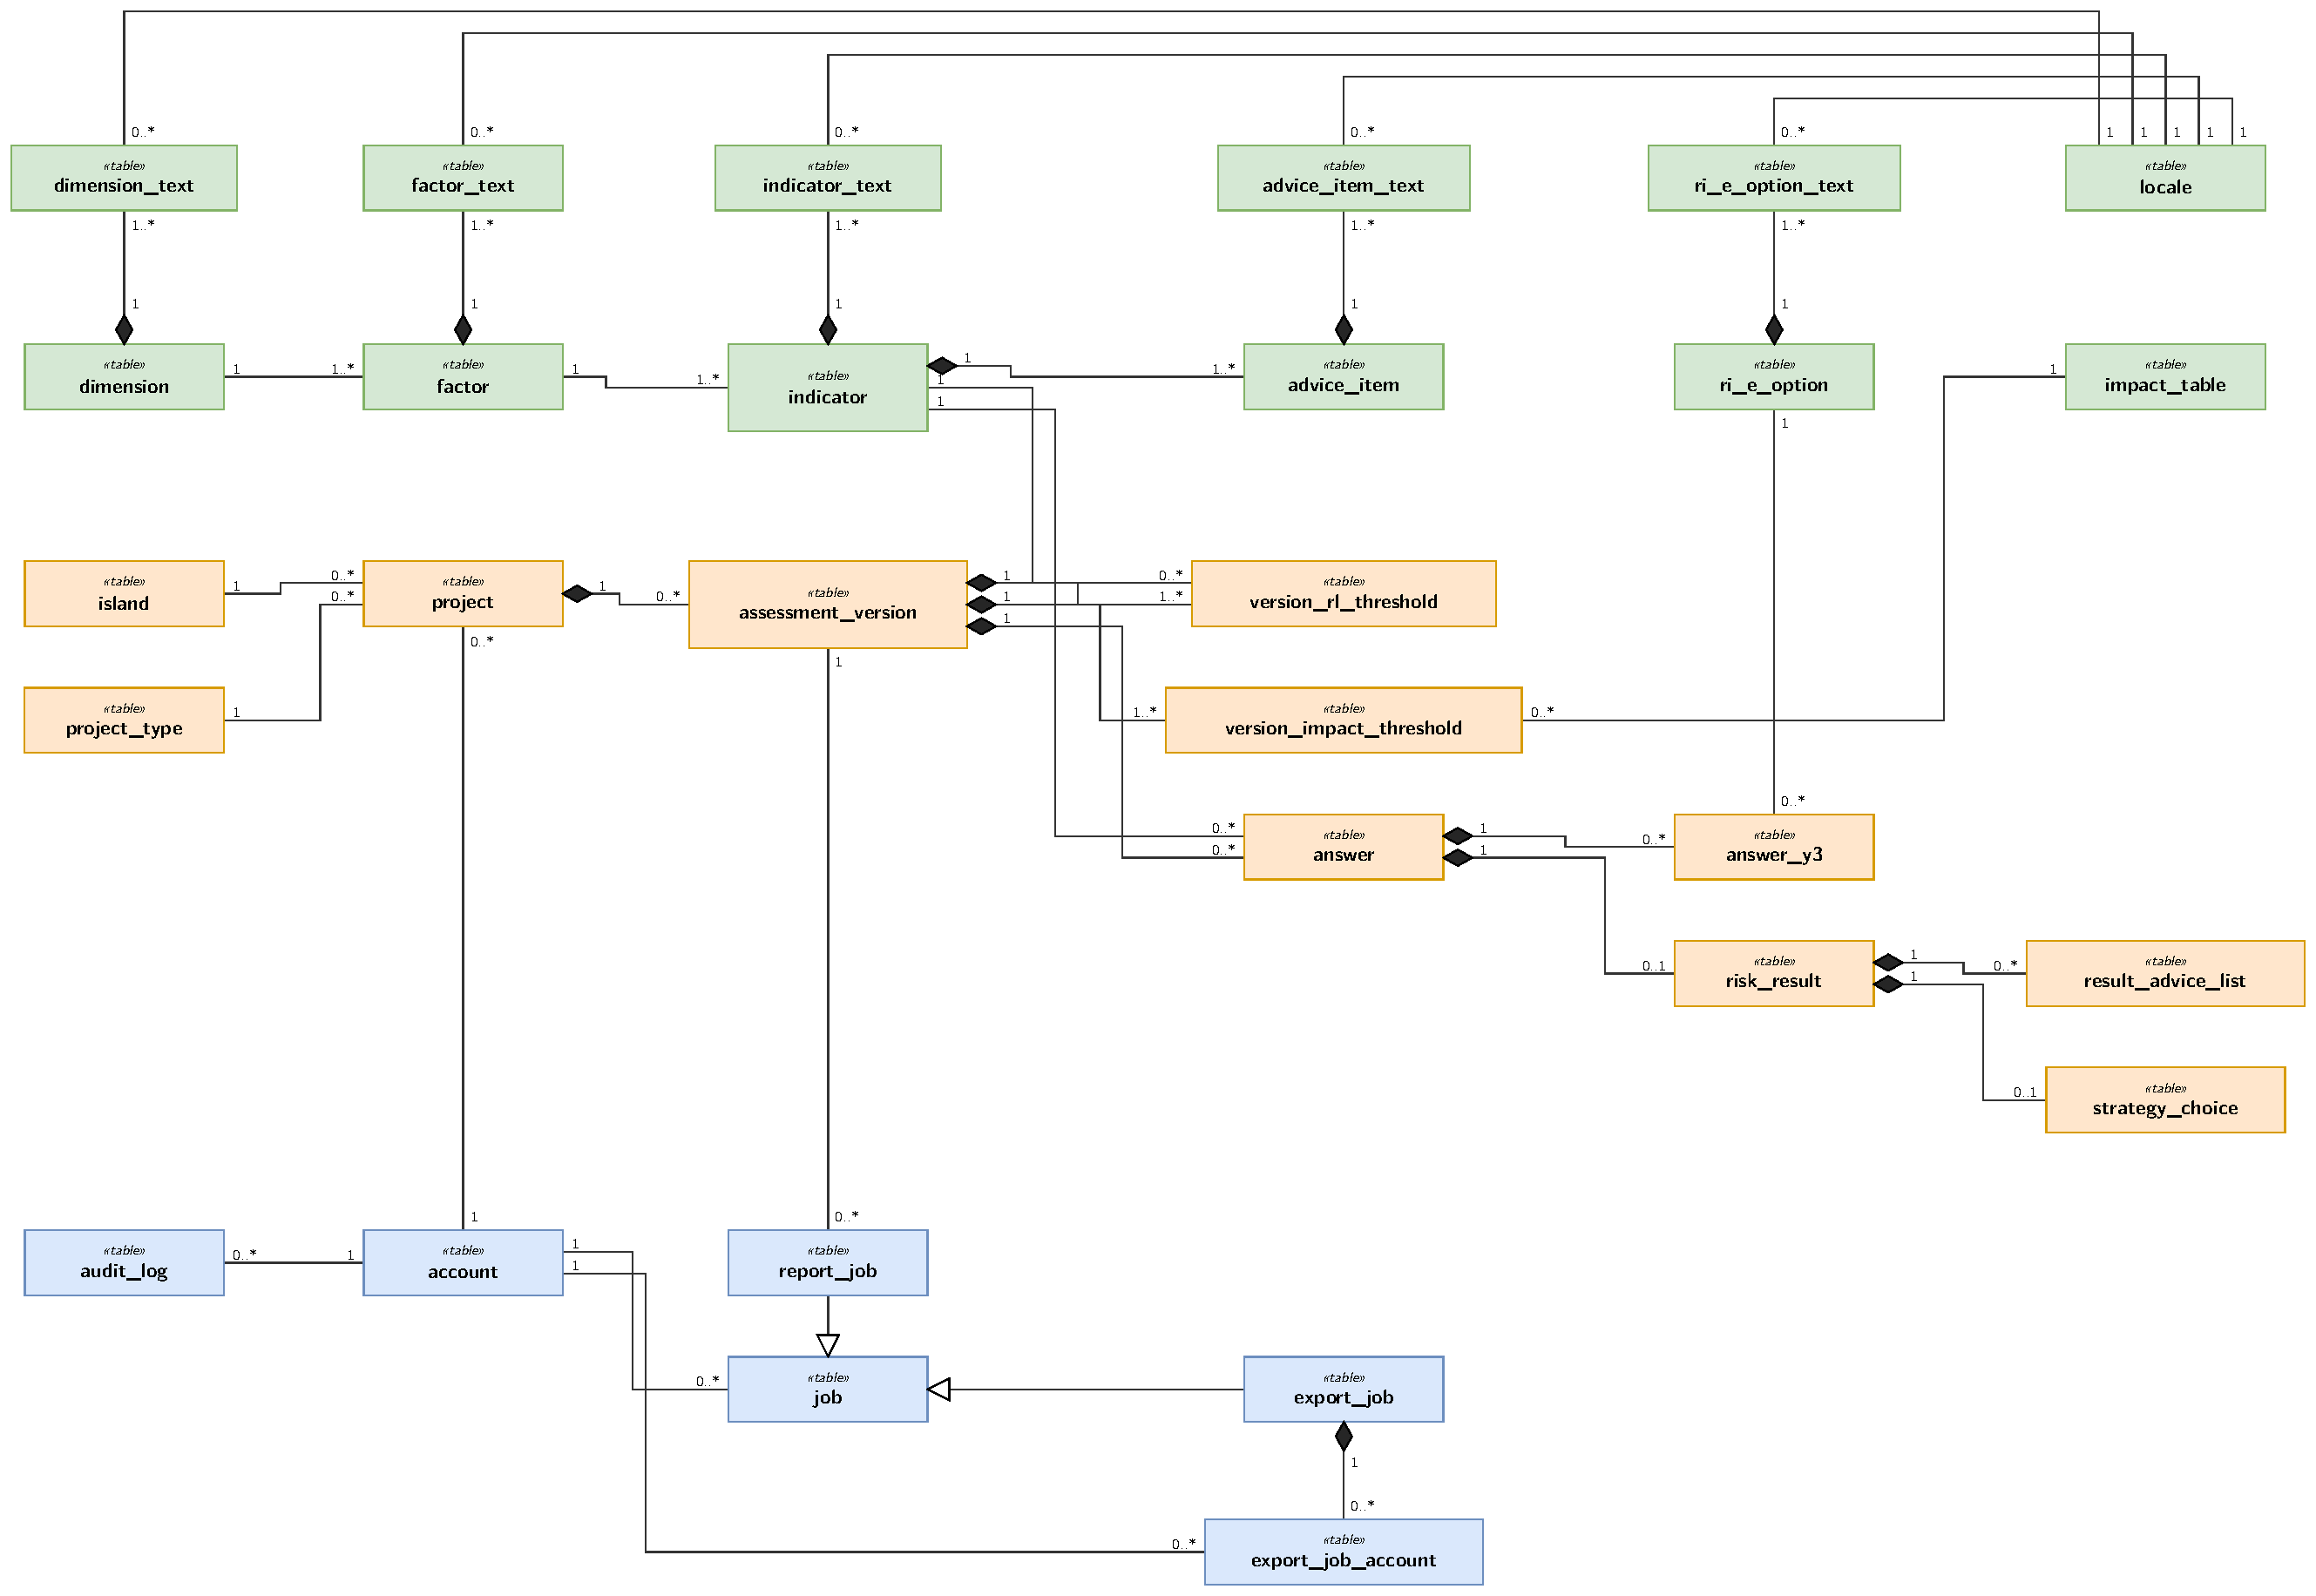
\includegraphics[width=\linewidth,height=0.9\textheight,keepaspectratio]{figures/er-overview.pdf}
\caption{UML ER overview: all 29 entities and their relationships. The three \tb{updated\_by} links from the catalogue to \tb{account} are shown in Figure~\ref{fig:cat} only.}
\label{fig:overview}
\end{figure}
\begin{figure}[p]
\centering
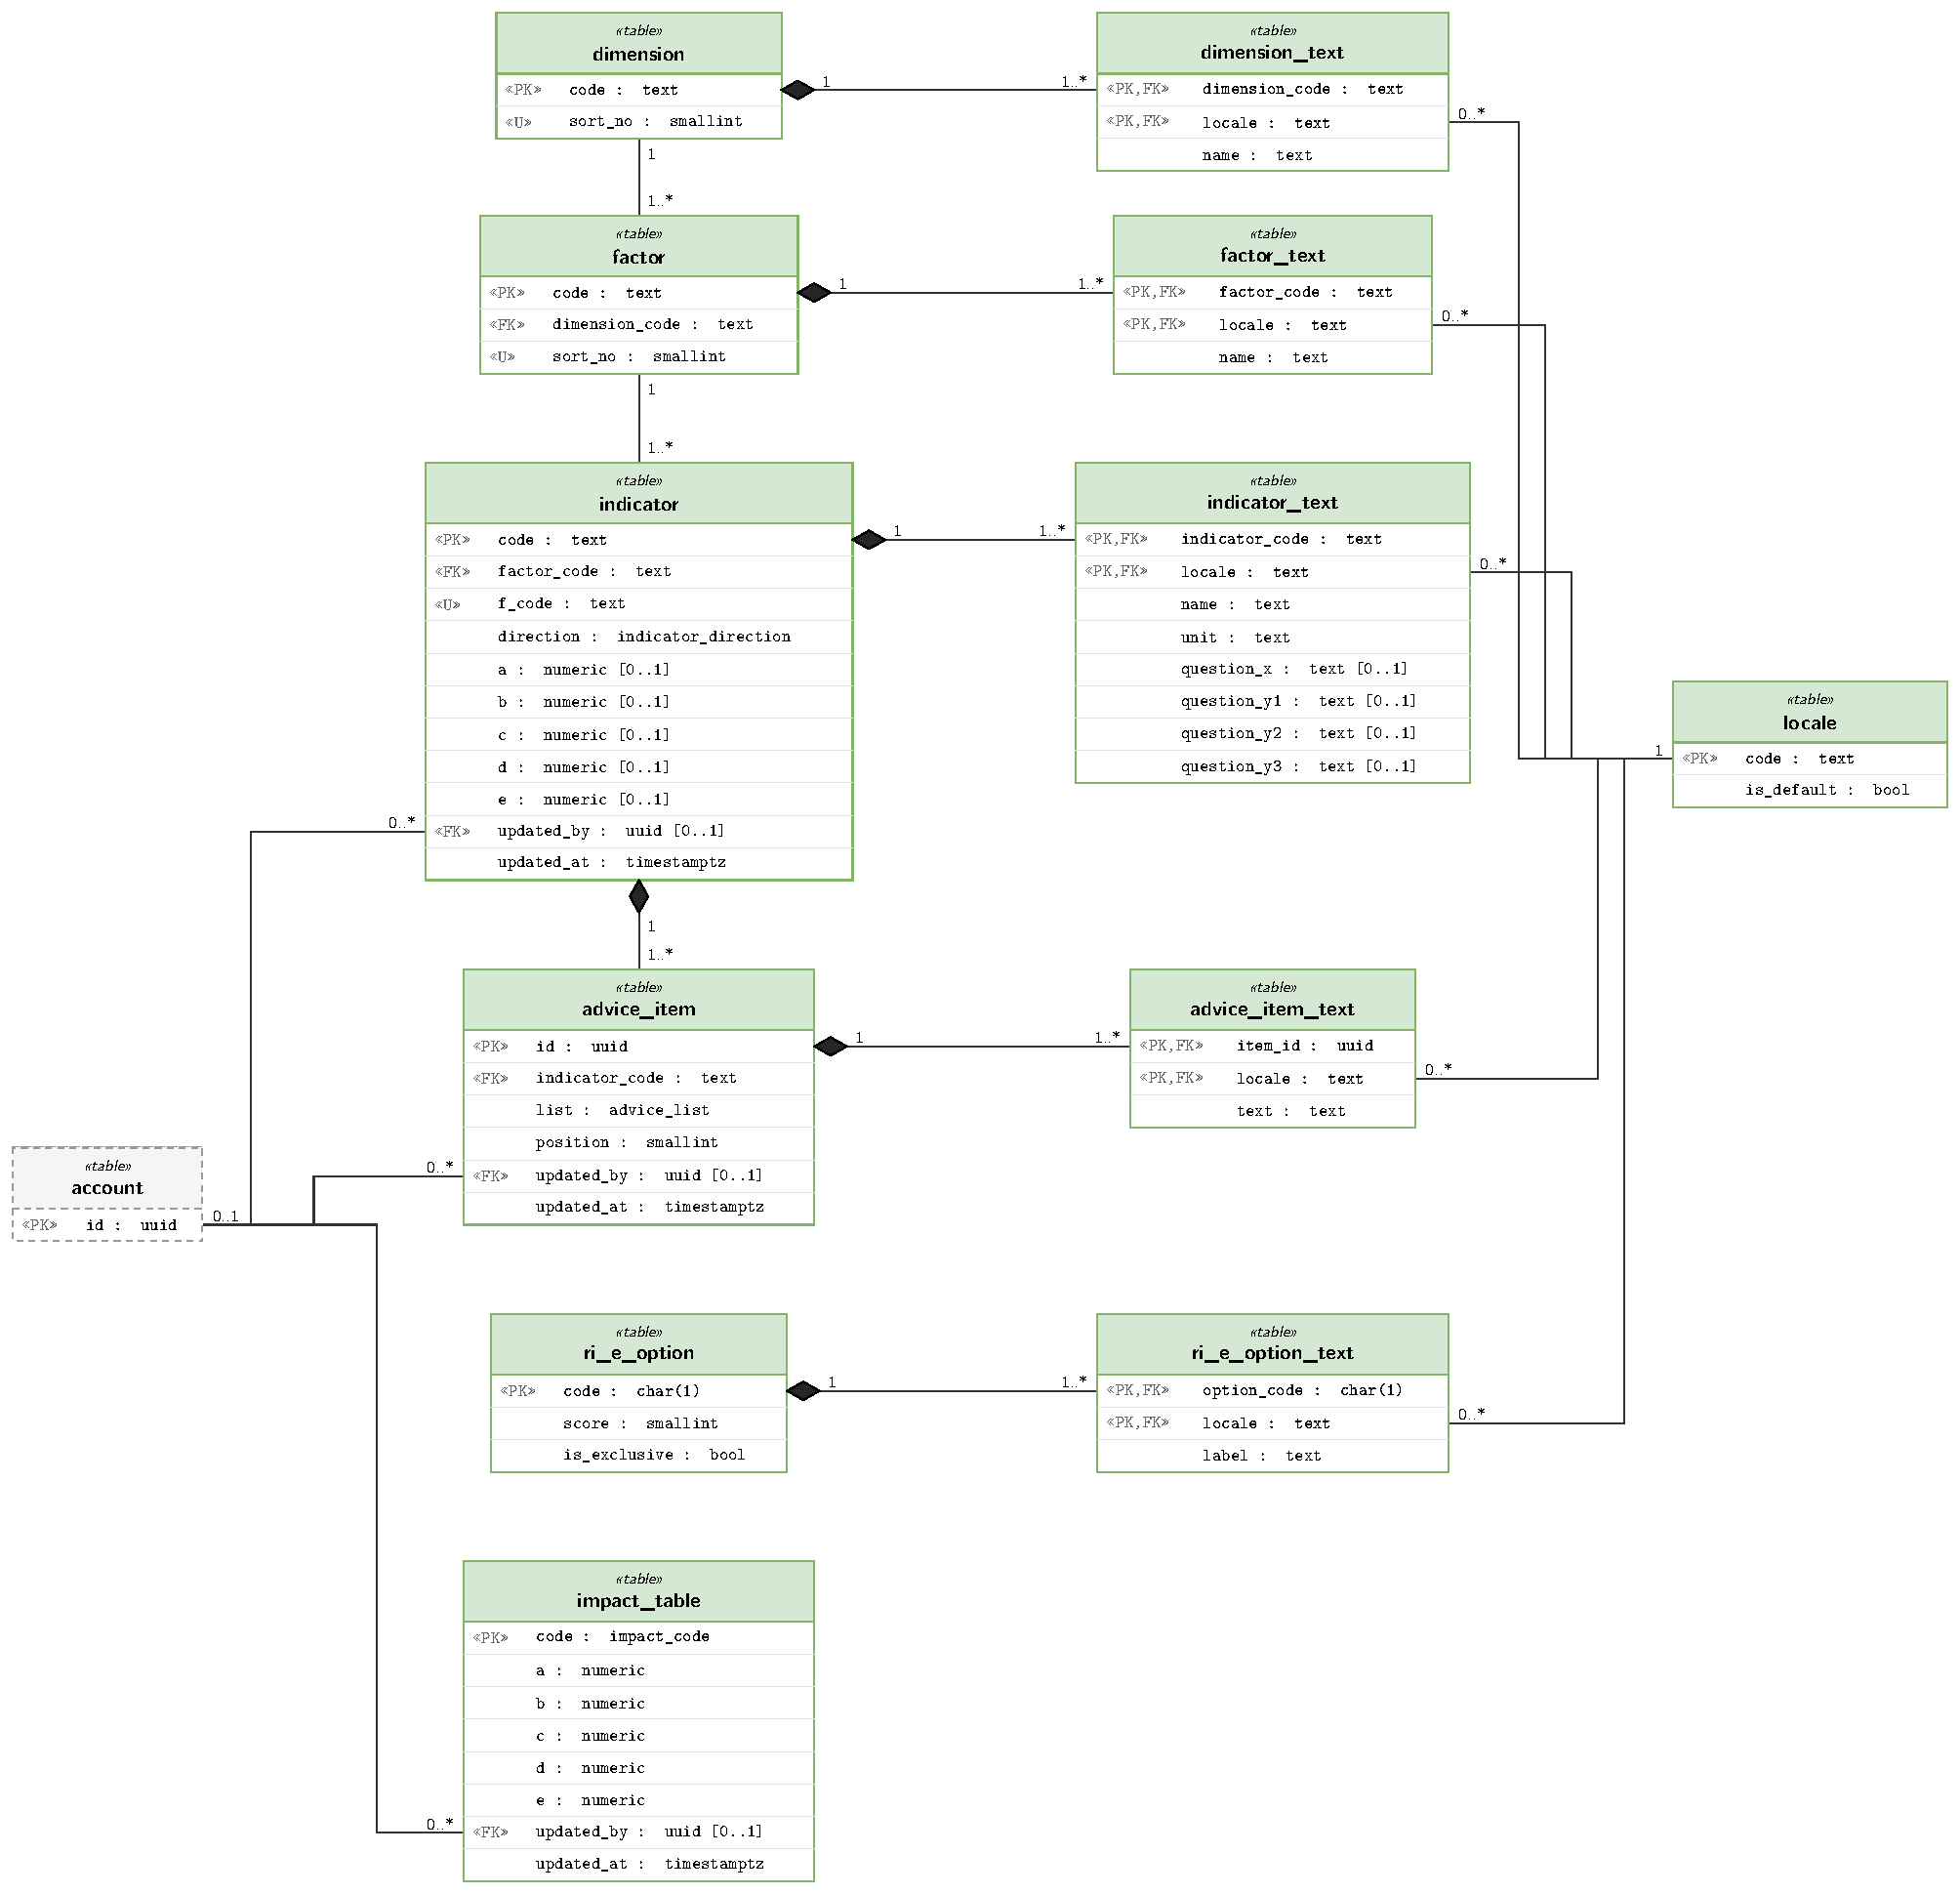
\includegraphics[width=\linewidth,height=0.93\textheight,keepaspectratio]{figures/er-catalogue.pdf}
\caption{Indicator catalogue.}
\label{fig:cat}
\end{figure}
\begin{figure}[p]
\centering
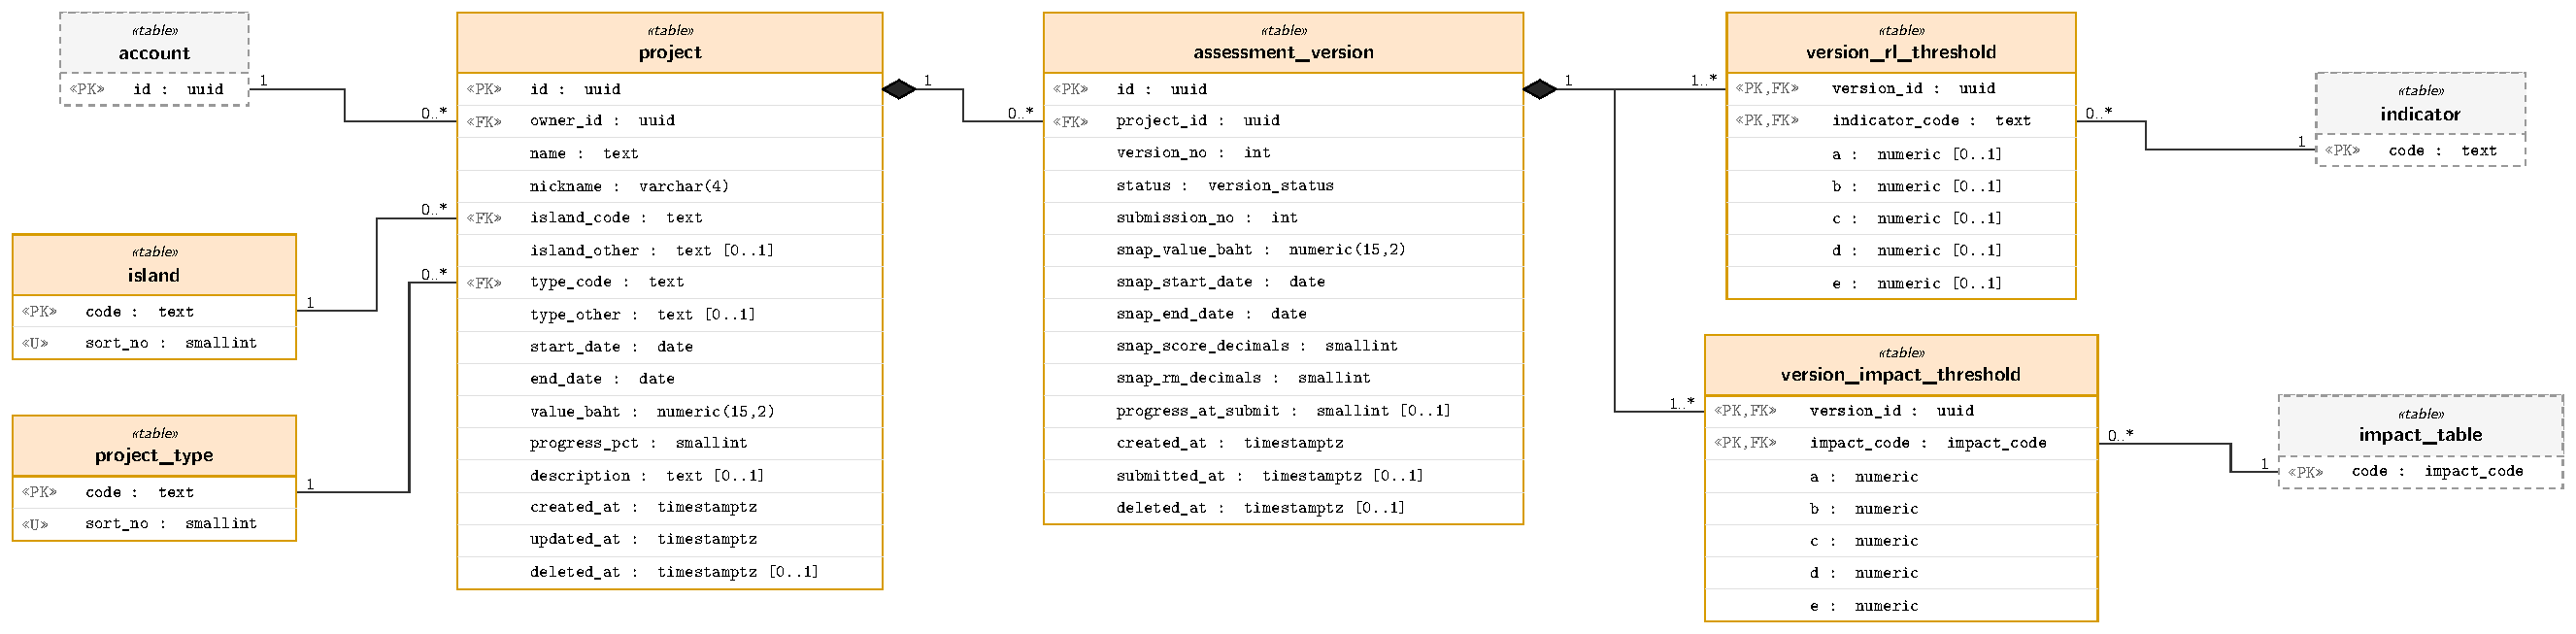
\includegraphics[width=\linewidth]{figures/er-projects.pdf}
\caption{Projects and versions, with the per-version snapshot.}
\label{fig:prj}
\vspace{8pt}
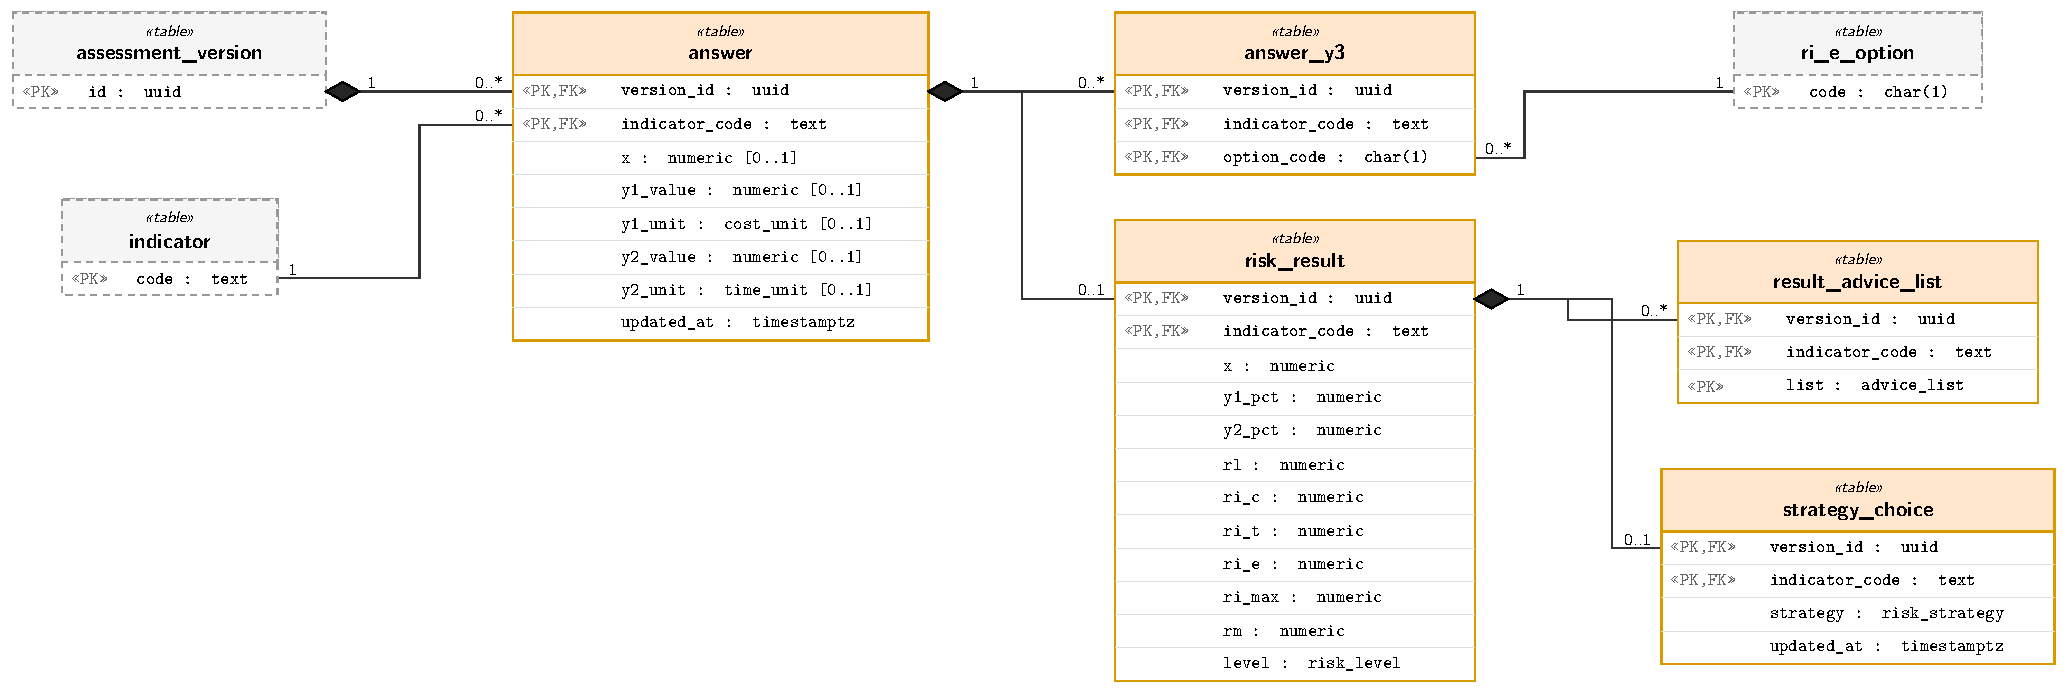
\includegraphics[width=\linewidth]{figures/er-assessments.pdf}
\caption{Answers and results.}
\label{fig:res}
\end{figure}
\begin{figure}[p]
\centering
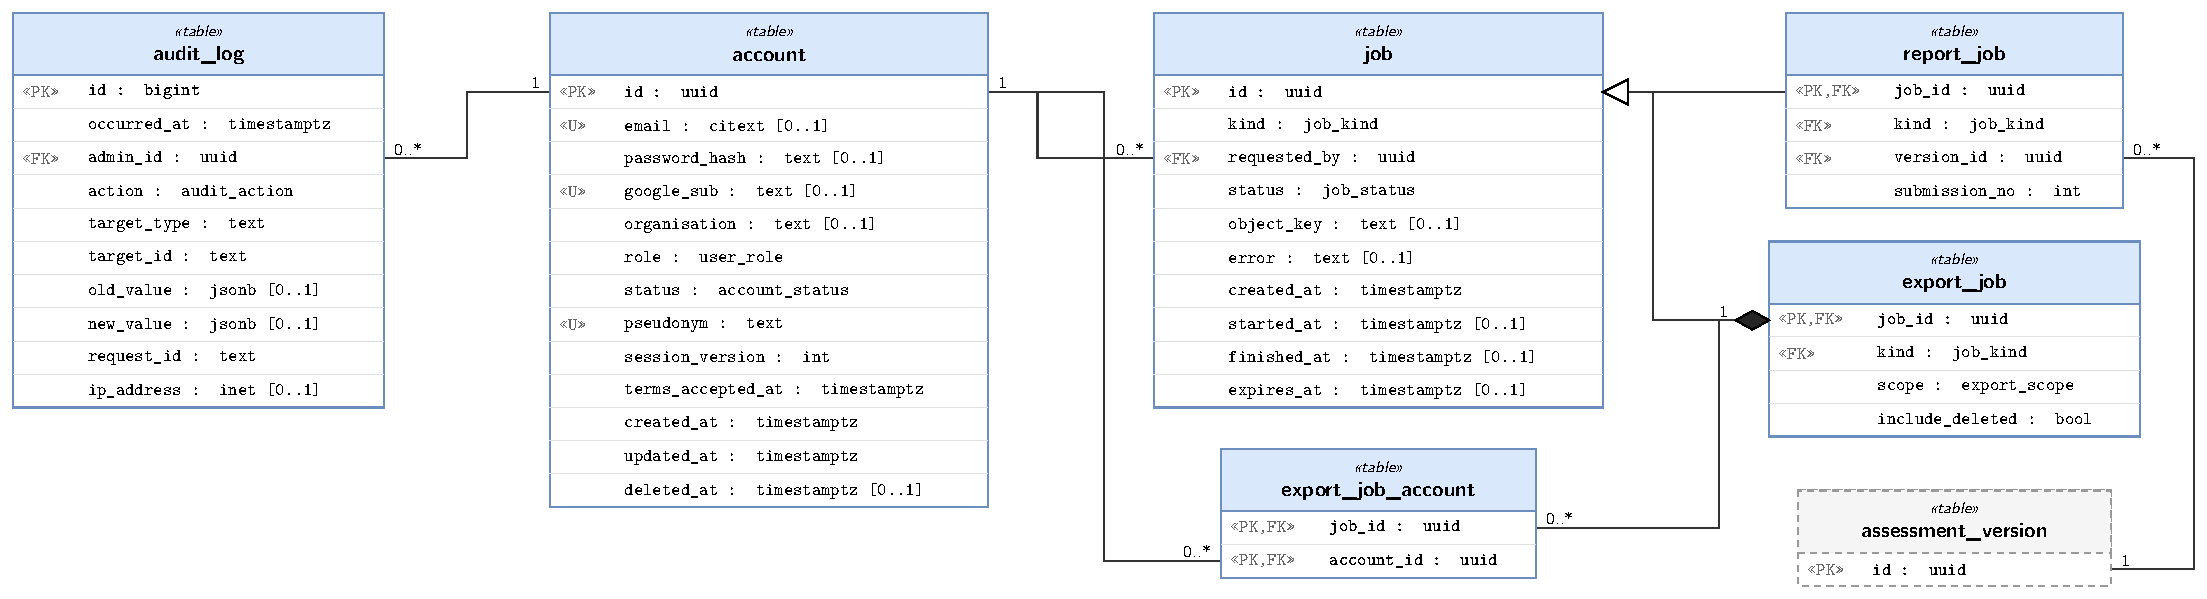
\includegraphics[width=\linewidth]{figures/er-accounts.pdf}
\caption{Accounts, jobs and audit log.}
\label{fig:acc}
\end{figure}
\end{landscape}

%------------------------------------------------------------
\needspace{0.5\textheight}\section{Normalisation}

The schema is in Boyce–Codd normal form (BCNF): in every table, each non-trivial functional dependency has a candidate key on its left side. The steps below show where the requirements, read naively, would break a normal form and how the model avoids it.

\noindent\textbf{First normal form (atomic values, no repeating groups).}
\begin{itemize}
\item $y_3$ is a multi-select of options A--I, so it is not a column of \tb{answer}: each ticked option is a row of \tb{answer\_y3}.
\item Advice lists hold 1--5 items, so items are rows of \tb{advice\_item} (one per indicator, list and position), not an array column.
\item The advice lists selected for a result (1--3) are rows of \tb{result\_advice\_list}, and the users selected for an export are rows of \tb{export\_job\_account}.
\item Texts in several languages are rows of the \tb{*\_text} tables, not \tb{name\_th} / \tb{name\_en} columns. Adding \tb{en} then needs no schema change (FR-55, FR-56).
\item The version snapshot is stored as rows (\tb{version\_rl\_threshold}, \tb{version\_impact\_threshold}) and columns of \tb{assessment\_version}, not as one JSON document (\S\ref{sec:changes}).
\end{itemize}

\noindent\textbf{Second normal form (no partial dependency on a composite key).}
\begin{itemize}
\item \tb{answer} has the key (\tb{version\_id}, \tb{indicator\_code}). The project value, dates and rounding settings depend on \tb{version\_id} alone, so they live on \tb{assessment\_version}, not on each answer or result. Storing the rounding settings on each result, as the architecture decisions suggest, would break 2NF in the same way (\S\ref{sec:changes}).
\item In the \tb{*\_text} tables, names and questions depend on the whole key (entity, locale). The factor of an indicator depends on the indicator alone, so it stays on \tb{indicator}.
\end{itemize}

\noindent\textbf{Third normal form and BCNF (no transitive dependency).}
\begin{itemize}
\item \tb{project} stores \tb{island\_code}; the island's label depends on the code, so it is not copied into the project.
\item The dimension of an indicator follows from its factor, so \tb{indicator} has \tb{factor\_code} only.
\item Report and export jobs have different attributes. One job table with nullable columns for both would make those columns depend on \tb{kind}; instead \tb{report\_job} and \tb{export\_job} are subtypes of \tb{job}.
\item $y_1$ and $y_2$ in \% follow from the entered value, the unit and the version snapshot, so \tb{answer} keeps only the entered value and unit. The \% values used by the engine are stored once, on \tb{risk\_result}.
\item Values that are only computed from other rows are not stored: the latest version of a project (\tb{max(version\_no)}), expected progress (BR-24), dashboard figures (BR-26) and per-user project and version counts.
\end{itemize}

\subsection{Controlled redundancy}
A few stored values could be derived. Each is kept on purpose and guarded so it cannot drift from its source.

{\small
\begin{longtable}{@{}R{4.6cm} R{7.4cm} R{4.1cm}@{}}
\toprule\rowcolor{hdr}Stored value & Why it is stored & Guard \\ \midrule\endhead
Snapshot columns and tables of a version & Not a copy of current data but a historical fact: what the project and thresholds were when the version was created (BR-10). Later edits must not change old scores. & Written once in the version's creating transaction; no update path. \\
\tb{risk\_result.ri\_max}, \tb{rm}, \tb{level} & Results, PDF and export read the stored results; nothing is recalculated on read (AD). The score inputs are also stored, so each result can be audited. & \tb{ri\_max} and \tb{level} checks; scores in [1, 5]. \\
\tb{assessment\_version.status} & Follows from \tb{submission\_no} (0 = draft), but reads more clearly in queries and the API. & Check ties both together with \tb{submitted\_at}. \\
\tb{kind} in \tb{report\_job} and \tb{export\_job} & Lets a foreign key prove that a report row hangs on a report job (disjoint subtypes) without triggers. & FK to \tb{job(id, kind)} and a constant check. \\
\tb{audit\_log.old\_value}, \tb{new\_value} (\tb{jsonb}) & Each target type has a different shape (a user's role, a list of advice items, five thresholds). The log keeps an immutable copy for humans, not data the application queries by field. & Written in the same transaction as the change; application role has \textsc{insert} and \textsc{select} only. \\
\bottomrule
\end{longtable}}

\subsection{Changes to Architecture Decisions v2.10}\label{sec:changes}
\begin{enumerate}
\item \textbf{Snapshot as rows, not one JSON document.} Same content (project value, dates, all RL thresholds, $\RIC$/$\RIT$ tables, $p_s$, $p_m$), now typed and checked. The research export still writes it as JSON in \tb{project.json}.
\item \textbf{Rounding settings stored per version, not per result.} A version's settings never change after creation, so storing them on every result would repeat the same value 55 times.
\item \textbf{\% of $y_1$, $y_2$ stored on the result, not on the answer.} The answer keeps what the user entered; the result keeps the engine inputs used at the last submission.
\end{enumerate}

%------------------------------------------------------------
\needspace{0.5\textheight}\section{Database Schema}\label{sec:schema}

Each table lists its columns in order. \emph{Null} = yes marks a nullable column; \emph{Key} gives the primary key (PK), foreign keys (FK $\to$ parent table, referencing its primary key) and single-column unique keys (U). Composite keys appear as PK on each of their columns. Checks over several columns follow the table. Foreign keys are \textsc{on delete restrict} unless marked \textsc{cascade}: in normal use only advice items, answers' $y_3$ options and results are ever deleted.

\subsection{Enumerated types}
{\small
\begin{tabularx}{\linewidth}{@{}>{\ttfamily}l Y@{}}
\toprule\rowcolor{hdr}\normalfont Type & Values \\ \midrule
user\_role & \texttt{user}, \texttt{admin} \\
account\_status & \texttt{active}, \texttt{deactivated}, \texttt{deleted} \\
indicator\_direction & \texttt{normal}, \texttt{inverse} \\
impact\_code & \texttt{RI\_C}, \texttt{RI\_T} \\
advice\_list & \texttt{RL}, \texttt{RI\_C}, \texttt{RI\_T}, \texttt{RI\_E} \\
version\_status & \texttt{draft}, \texttt{submitted} \\
cost\_unit & \texttt{baht}, \texttt{percent} \\
time\_unit & \texttt{day}, \texttt{percent} \\
risk\_level & \texttt{VL}, \texttt{L}, \texttt{M}, \texttt{H}, \texttt{VH} \\
risk\_strategy & \texttt{REDUCE}, \texttt{TRANSFER}, \texttt{AVOID}, \texttt{ACCEPT} \\
job\_kind & \texttt{report}, \texttt{export} \\
job\_status & \texttt{queued}, \texttt{running}, \texttt{done}, \texttt{failed}, \texttt{expired} \\
export\_scope & \texttt{all}, \texttt{selected} \\
audit\_action & \texttt{user\_role\_change}, \texttt{user\_deactivate}, \texttt{user\_reactivate}, \texttt{user\_delete}, \texttt{advice\_edit}, \texttt{rl\_threshold\_edit}, \texttt{impact\_table\_edit}, \texttt{export\_request}, \texttt{export\_download} \\
\bottomrule
\end{tabularx}}

\needspace{12\baselineskip}\subsection{Indicator catalogue}
\needspace{8\baselineskip}
\subsubsection*{\texttt{locale}}
\noindent Supported content locales.\par\vspace{2pt}
{\footnotesize\setlength{\tabcolsep}{4pt}\noindent\begin{tabularx}{\linewidth}{@{}>{\ttfamily\raggedright\arraybackslash}p{3.2cm} >{\ttfamily\raggedright\arraybackslash}p{3.15cm} >{\centering\arraybackslash}p{0.6cm} >{\raggedright\arraybackslash}p{3.85cm} Y@{}}
\toprule\rowcolor{hdr}\normalfont Column & \normalfont Type & Null & Key & Rule \\ \midrule
code & text &  & PK & Two lower-case letters: \texttt{th}, \texttt{en}. \\
is\_default & bool &  &  & Exactly one default (\texttt{th}); partial unique index. \\
\bottomrule\end{tabularx}}

\needspace{8\baselineskip}
\subsubsection*{\texttt{dimension}}
\noindent Risk dimensions (3).\par\vspace{2pt}
{\footnotesize\setlength{\tabcolsep}{4pt}\noindent\begin{tabularx}{\linewidth}{@{}>{\ttfamily\raggedright\arraybackslash}p{3.2cm} >{\ttfamily\raggedright\arraybackslash}p{3.15cm} >{\centering\arraybackslash}p{0.6cm} >{\raggedright\arraybackslash}p{3.85cm} Y@{}}
\toprule\rowcolor{hdr}\normalfont Column & \normalfont Type & Null & Key & Rule \\ \midrule
code & text &  & PK & \texttt{EC}, \texttt{SO}, \texttt{EV}. \\
sort\_no & smallint &  & U &  \\
\bottomrule\end{tabularx}}

\needspace{9\baselineskip}
\subsubsection*{\texttt{dimension\_text}}
\noindent Dimension names per locale.\par\vspace{2pt}
{\footnotesize\setlength{\tabcolsep}{4pt}\noindent\begin{tabularx}{\linewidth}{@{}>{\ttfamily\raggedright\arraybackslash}p{3.2cm} >{\ttfamily\raggedright\arraybackslash}p{3.15cm} >{\centering\arraybackslash}p{0.6cm} >{\raggedright\arraybackslash}p{3.85cm} Y@{}}
\toprule\rowcolor{hdr}\normalfont Column & \normalfont Type & Null & Key & Rule \\ \midrule
dimension\_code & text &  & PK, FK$\to$\texttt{dimension} &  \\
locale & text &  & PK, FK$\to$\texttt{locale} &  \\
name & text &  &  &  \\
\bottomrule\end{tabularx}}

\needspace{9\baselineskip}
\subsubsection*{\texttt{factor}}
\noindent Risk factors (11).\par\vspace{2pt}
{\footnotesize\setlength{\tabcolsep}{4pt}\noindent\begin{tabularx}{\linewidth}{@{}>{\ttfamily\raggedright\arraybackslash}p{3.2cm} >{\ttfamily\raggedright\arraybackslash}p{3.15cm} >{\centering\arraybackslash}p{0.6cm} >{\raggedright\arraybackslash}p{3.85cm} Y@{}}
\toprule\rowcolor{hdr}\normalfont Column & \normalfont Type & Null & Key & Rule \\ \midrule
code & text &  & PK & e.g.\ \texttt{EC-MG}. \\
dimension\_code & text &  & FK$\to$\texttt{dimension} &  \\
sort\_no & smallint &  & U &  \\
\bottomrule\end{tabularx}}

\needspace{9\baselineskip}
\subsubsection*{\texttt{factor\_text}}
\noindent Factor names per locale.\par\vspace{2pt}
{\footnotesize\setlength{\tabcolsep}{4pt}\noindent\begin{tabularx}{\linewidth}{@{}>{\ttfamily\raggedright\arraybackslash}p{3.2cm} >{\ttfamily\raggedright\arraybackslash}p{3.15cm} >{\centering\arraybackslash}p{0.6cm} >{\raggedright\arraybackslash}p{3.85cm} Y@{}}
\toprule\rowcolor{hdr}\normalfont Column & \normalfont Type & Null & Key & Rule \\ \midrule
factor\_code & text &  & PK, FK$\to$\texttt{factor} &  \\
locale & text &  & PK, FK$\to$\texttt{locale} &  \\
name & text &  &  &  \\
\bottomrule\end{tabularx}}

\needspace{18\baselineskip}
\subsubsection*{\texttt{indicator}}
\noindent Risk indicators (55) with their current RL thresholds.\par\vspace{2pt}
{\footnotesize\setlength{\tabcolsep}{4pt}\noindent\begin{tabularx}{\linewidth}{@{}>{\ttfamily\raggedright\arraybackslash}p{3.2cm} >{\ttfamily\raggedright\arraybackslash}p{3.15cm} >{\centering\arraybackslash}p{0.6cm} >{\raggedright\arraybackslash}p{3.85cm} Y@{}}
\toprule\rowcolor{hdr}\normalfont Column & \normalfont Type & Null & Key & Rule \\ \midrule
code & text &  & PK & e.g.\ \texttt{EC-MG-1}. \\
factor\_code & text &  & FK$\to$\texttt{factor} &  \\
f\_code & text &  & U & Research code, e.g.\ \texttt{F11}. \\
direction & indicator\_direction &  &  & \texttt{inverse} for EC-MG-5, EC-CO-5, EC-RS-1, EV-EV-4. \\
a & numeric & yes &  & RL thresholds; NULL = not used. See table checks. \\
b & numeric & yes &  &  \\
c & numeric & yes &  &  \\
d & numeric & yes &  &  \\
e & numeric & yes &  &  \\
updated\_by & uuid & yes & FK$\to$\texttt{account} & NULL for seeded values. \\
updated\_at & timestamptz &  &  & Default \texttt{now()}. \\
\bottomrule\end{tabularx}}
{\footnotesize\noindent\textit{Table checks:} Pattern: all of $a..e$, only $a,b,c$, or only $c,d,e$ set. Set values $\ge 0$; strictly increasing (\texttt{normal}) or strictly decreasing (\texttt{inverse}).\par}

\needspace{13\baselineskip}
\subsubsection*{\texttt{indicator\_text}}
\noindent Indicator name, unit and the four questions per locale.\par\vspace{2pt}
{\footnotesize\setlength{\tabcolsep}{4pt}\noindent\begin{tabularx}{\linewidth}{@{}>{\ttfamily\raggedright\arraybackslash}p{3.2cm} >{\ttfamily\raggedright\arraybackslash}p{3.15cm} >{\centering\arraybackslash}p{0.6cm} >{\raggedright\arraybackslash}p{3.85cm} Y@{}}
\toprule\rowcolor{hdr}\normalfont Column & \normalfont Type & Null & Key & Rule \\ \midrule
indicator\_code & text &  & PK, FK$\to$\texttt{indicator} &  \\
locale & text &  & PK, FK$\to$\texttt{locale} &  \\
name & text &  &  &  \\
unit & text &  &  &  \\
question\_x & text & yes &  & Required in the \texttt{th} row (seed check). \\
question\_y1 & text & yes &  &  \\
question\_y2 & text & yes &  &  \\
question\_y3 & text & yes &  &  \\
\bottomrule\end{tabularx}}

\needspace{9\baselineskip}
\subsubsection*{\texttt{ri\_e\_option}}
\noindent Environmental impact options A--I and their fixed scores.\par\vspace{2pt}
{\footnotesize\setlength{\tabcolsep}{4pt}\noindent\begin{tabularx}{\linewidth}{@{}>{\ttfamily\raggedright\arraybackslash}p{3.2cm} >{\ttfamily\raggedright\arraybackslash}p{3.15cm} >{\centering\arraybackslash}p{0.6cm} >{\raggedright\arraybackslash}p{3.85cm} Y@{}}
\toprule\rowcolor{hdr}\normalfont Column & \normalfont Type & Null & Key & Rule \\ \midrule
code & char(1) &  & PK & \texttt{A}--\texttt{I}. \\
score & smallint &  &  & 1--5; fixed, no admin UI. \\
is\_exclusive & bool &  &  & True for \texttt{A}: cannot be combined. \\
\bottomrule\end{tabularx}}

\needspace{9\baselineskip}
\subsubsection*{\texttt{ri\_e\_option\_text}}
\noindent Option labels per locale.\par\vspace{2pt}
{\footnotesize\setlength{\tabcolsep}{4pt}\noindent\begin{tabularx}{\linewidth}{@{}>{\ttfamily\raggedright\arraybackslash}p{3.2cm} >{\ttfamily\raggedright\arraybackslash}p{3.15cm} >{\centering\arraybackslash}p{0.6cm} >{\raggedright\arraybackslash}p{3.85cm} Y@{}}
\toprule\rowcolor{hdr}\normalfont Column & \normalfont Type & Null & Key & Rule \\ \midrule
option\_code & char(1) &  & PK, FK$\to$\texttt{ri\_e\_option} &  \\
locale & text &  & PK, FK$\to$\texttt{locale} &  \\
label & text &  &  &  \\
\bottomrule\end{tabularx}}

\needspace{15\baselineskip}
\subsubsection*{\texttt{impact\_table}}
\noindent Shared $\RIC$ and $\RIT$ threshold tables.\par\vspace{2pt}
{\footnotesize\setlength{\tabcolsep}{4pt}\noindent\begin{tabularx}{\linewidth}{@{}>{\ttfamily\raggedright\arraybackslash}p{3.2cm} >{\ttfamily\raggedright\arraybackslash}p{3.15cm} >{\centering\arraybackslash}p{0.6cm} >{\raggedright\arraybackslash}p{3.85cm} Y@{}}
\toprule\rowcolor{hdr}\normalfont Column & \normalfont Type & Null & Key & Rule \\ \midrule
code & impact\_code &  & PK &  \\
a & numeric &  &  & All five set; $0 \le a < b < c < d < e$. \\
b & numeric &  &  &  \\
c & numeric &  &  &  \\
d & numeric &  &  &  \\
e & numeric &  &  &  \\
updated\_by & uuid & yes & FK$\to$\texttt{account} &  \\
updated\_at & timestamptz &  &  & Default \texttt{now()}. \\
\bottomrule\end{tabularx}}
{\footnotesize\noindent\textit{Table checks:} $0 \le a < b < c < d < e$.\par}

\needspace{14\baselineskip}
\subsubsection*{\texttt{advice\_item}}
\noindent One advice item of one list of one indicator.\par\vspace{2pt}
{\footnotesize\setlength{\tabcolsep}{4pt}\noindent\begin{tabularx}{\linewidth}{@{}>{\ttfamily\raggedright\arraybackslash}p{3.2cm} >{\ttfamily\raggedright\arraybackslash}p{3.15cm} >{\centering\arraybackslash}p{0.6cm} >{\raggedright\arraybackslash}p{3.85cm} Y@{}}
\toprule\rowcolor{hdr}\normalfont Column & \normalfont Type & Null & Key & Rule \\ \midrule
id & uuid &  & PK &  \\
indicator\_code & text &  & FK$\to$\texttt{indicator} &  \\
list & advice\_list &  &  & Which score the item belongs to. \\
position & smallint &  &  & 1--5; unique per (indicator, list), deferrable for reordering. \\
updated\_by & uuid & yes & FK$\to$\texttt{account} &  \\
updated\_at & timestamptz &  &  & Default \texttt{now()}. \\
\bottomrule\end{tabularx}}
{\footnotesize\noindent\textit{Table checks:} \textsc{unique} (\texttt{indicator\_code, list, position}) \textsc{deferrable}.\par}

\needspace{9\baselineskip}
\subsubsection*{\texttt{advice\_item\_text}}
\noindent Advice text per locale.\par\vspace{2pt}
{\footnotesize\setlength{\tabcolsep}{4pt}\noindent\begin{tabularx}{\linewidth}{@{}>{\ttfamily\raggedright\arraybackslash}p{3.2cm} >{\ttfamily\raggedright\arraybackslash}p{3.15cm} >{\centering\arraybackslash}p{0.6cm} >{\raggedright\arraybackslash}p{3.85cm} Y@{}}
\toprule\rowcolor{hdr}\normalfont Column & \normalfont Type & Null & Key & Rule \\ \midrule
item\_id & uuid &  & PK, FK$\to$\texttt{advice\_item} & \textsc{on delete cascade}. \\
locale & text &  & PK, FK$\to$\texttt{locale} &  \\
text & text &  &  & Not blank. \texttt{th} row required. \\
\bottomrule\end{tabularx}}

\needspace{12\baselineskip}\subsection{Projects and assessments}
\needspace{8\baselineskip}
\subsubsection*{\texttt{island}}
\noindent Island / location codes.\par\vspace{2pt}
{\footnotesize\setlength{\tabcolsep}{4pt}\noindent\begin{tabularx}{\linewidth}{@{}>{\ttfamily\raggedright\arraybackslash}p{3.2cm} >{\ttfamily\raggedright\arraybackslash}p{3.15cm} >{\centering\arraybackslash}p{0.6cm} >{\raggedright\arraybackslash}p{3.85cm} Y@{}}
\toprule\rowcolor{hdr}\normalfont Column & \normalfont Type & Null & Key & Rule \\ \midrule
code & text &  & PK & \texttt{koh\_tao} \dots\ \texttt{koh\_kood}, \texttt{other}. Labels in message catalogues. \\
sort\_no & smallint &  & U &  \\
\bottomrule\end{tabularx}}

\needspace{8\baselineskip}
\subsubsection*{\texttt{project\_type}}
\noindent Project type codes.\par\vspace{2pt}
{\footnotesize\setlength{\tabcolsep}{4pt}\noindent\begin{tabularx}{\linewidth}{@{}>{\ttfamily\raggedright\arraybackslash}p{3.2cm} >{\ttfamily\raggedright\arraybackslash}p{3.15cm} >{\centering\arraybackslash}p{0.6cm} >{\raggedright\arraybackslash}p{3.85cm} Y@{}}
\toprule\rowcolor{hdr}\normalfont Column & \normalfont Type & Null & Key & Rule \\ \midrule
code & text &  & PK & \texttt{building}, \texttt{pier}, \texttt{road}, \texttt{utilities}, \texttt{coastal}, \texttt{other}. \\
sort\_no & smallint &  & U &  \\
\bottomrule\end{tabularx}}

\needspace{22\baselineskip}
\subsubsection*{\texttt{project}}
\noindent A construction project owned by one account.\par\vspace{2pt}
{\footnotesize\setlength{\tabcolsep}{4pt}\noindent\begin{tabularx}{\linewidth}{@{}>{\ttfamily\raggedright\arraybackslash}p{3.2cm} >{\ttfamily\raggedright\arraybackslash}p{3.15cm} >{\centering\arraybackslash}p{0.6cm} >{\raggedright\arraybackslash}p{3.85cm} Y@{}}
\toprule\rowcolor{hdr}\normalfont Column & \normalfont Type & Null & Key & Rule \\ \midrule
id & uuid &  & PK &  \\
owner\_id & uuid &  & FK$\to$\texttt{account} &  \\
name & text &  &  & Not blank. \\
nickname & varchar(4) &  &  & 3--4 characters. \\
island\_code & text &  & FK$\to$\texttt{island} &  \\
island\_other & text & yes &  & Set iff \texttt{island\_code = other}. \\
type\_code & text &  & FK$\to$\texttt{project\_type} &  \\
type\_other & text & yes &  & Set iff \texttt{type\_code = other}. \\
start\_date & date &  &  &  \\
end\_date & date &  &  & $>$ \texttt{start\_date}. \\
value\_baht & numeric(15,2) &  &  & $> 0$. \\
progress\_pct & smallint &  &  & 0--100, default 0. \\
description & text & yes &  &  \\
created\_at & timestamptz &  &  & Default \texttt{now()}. \\
updated\_at & timestamptz &  &  & Default \texttt{now()}. \\
deleted\_at & timestamptz & yes &  & Soft delete; no restore. \\
\bottomrule\end{tabularx}}
{\footnotesize\noindent\textit{Table checks:} \texttt{end\_date > start\_date}; \texttt{*\_other} set iff code is \texttt{other}.\par}

\needspace{20\baselineskip}
\subsubsection*{\texttt{assessment\_version}}
\noindent Version $v_n$ of a project, with the snapshot of project value, dates and rounding.\par\vspace{2pt}
{\footnotesize\setlength{\tabcolsep}{4pt}\noindent\begin{tabularx}{\linewidth}{@{}>{\ttfamily\raggedright\arraybackslash}p{3.2cm} >{\ttfamily\raggedright\arraybackslash}p{3.15cm} >{\centering\arraybackslash}p{0.6cm} >{\raggedright\arraybackslash}p{3.85cm} Y@{}}
\toprule\rowcolor{hdr}\normalfont Column & \normalfont Type & Null & Key & Rule \\ \midrule
id & uuid &  & PK &  \\
project\_id & uuid &  & FK$\to$\texttt{project} &  \\
version\_no & int &  &  & $\ge 1$; unique per project, never reused. \\
status & version\_status &  &  & Default \texttt{draft}. \\
submission\_no & int &  &  & Number of submissions; 0 = never submitted. \\
snap\_value\_baht & numeric(15,2) &  &  & Snapshot of the project at creation. \\
snap\_start\_date & date &  &  &  \\
snap\_end\_date & date &  &  & $>$ \texttt{snap\_start\_date}. \\
snap\_score\_decimals & smallint &  &  & $p_s$ from \texttt{SCORE\_DECIMALS}; 0--6. \\
snap\_rm\_decimals & smallint &  &  & $p_m$ from \texttt{RM\_DECIMALS}; 0--6. \\
progress\_at\_submit & smallint & yes &  & Project progress at the last submission. \\
created\_at & timestamptz &  &  & Default \texttt{now()}. \\
submitted\_at & timestamptz & yes &  &  \\
deleted\_at & timestamptz & yes &  & Soft delete; no restore. \\
\bottomrule\end{tabularx}}
{\footnotesize\noindent\textit{Table checks:} \textsc{unique} (\texttt{project\_id, version\_no}). Draft: \texttt{submission\_no = 0}, \texttt{submitted\_at} and \texttt{progress\_at\_submit} NULL. Submitted: \texttt{submission\_no > 0}, both set.\par}

\needspace{12\baselineskip}
\subsubsection*{\texttt{version\_rl\_threshold}}
\noindent Snapshot of every indicator's RL thresholds for a version.\par\vspace{2pt}
{\footnotesize\setlength{\tabcolsep}{4pt}\noindent\begin{tabularx}{\linewidth}{@{}>{\ttfamily\raggedright\arraybackslash}p{3.2cm} >{\ttfamily\raggedright\arraybackslash}p{3.15cm} >{\centering\arraybackslash}p{0.6cm} >{\raggedright\arraybackslash}p{3.85cm} Y@{}}
\toprule\rowcolor{hdr}\normalfont Column & \normalfont Type & Null & Key & Rule \\ \midrule
version\_id & uuid &  & PK, FK$\to$\texttt{assessment\_version} &  \\
indicator\_code & text &  & PK, FK$\to$\texttt{indicator} &  \\
a & numeric & yes &  & Copy of \texttt{indicator.a..e}; one row per indicator (55). \\
b & numeric & yes &  &  \\
c & numeric & yes &  &  \\
d & numeric & yes &  &  \\
e & numeric & yes &  &  \\
\bottomrule\end{tabularx}}

\needspace{12\baselineskip}
\subsubsection*{\texttt{version\_impact\_threshold}}
\noindent Snapshot of the $\RIC$/$\RIT$ tables for a version.\par\vspace{2pt}
{\footnotesize\setlength{\tabcolsep}{4pt}\noindent\begin{tabularx}{\linewidth}{@{}>{\ttfamily\raggedright\arraybackslash}p{3.2cm} >{\ttfamily\raggedright\arraybackslash}p{3.15cm} >{\centering\arraybackslash}p{0.6cm} >{\raggedright\arraybackslash}p{3.85cm} Y@{}}
\toprule\rowcolor{hdr}\normalfont Column & \normalfont Type & Null & Key & Rule \\ \midrule
version\_id & uuid &  & PK, FK$\to$\texttt{assessment\_version} &  \\
impact\_code & impact\_code &  & PK, FK$\to$\texttt{impact\_table} &  \\
a & numeric &  &  & Copy of \texttt{impact\_table}; two rows. \\
b & numeric &  &  &  \\
c & numeric &  &  &  \\
d & numeric &  &  &  \\
e & numeric &  &  &  \\
\bottomrule\end{tabularx}}

\needspace{15\baselineskip}
\subsubsection*{\texttt{answer}}
\noindent Answers of one indicator in one version, as entered.\par\vspace{2pt}
{\footnotesize\setlength{\tabcolsep}{4pt}\noindent\begin{tabularx}{\linewidth}{@{}>{\ttfamily\raggedright\arraybackslash}p{3.2cm} >{\ttfamily\raggedright\arraybackslash}p{3.15cm} >{\centering\arraybackslash}p{0.6cm} >{\raggedright\arraybackslash}p{3.85cm} Y@{}}
\toprule\rowcolor{hdr}\normalfont Column & \normalfont Type & Null & Key & Rule \\ \midrule
version\_id & uuid &  & PK, FK$\to$\texttt{assessment\_version} &  \\
indicator\_code & text &  & PK, FK$\to$\texttt{indicator} &  \\
x & numeric & yes &  & $\ge 0$, in the indicator unit. \\
y1\_value & numeric & yes &  & $\ge 0$; $\le 100$ when unit is \texttt{percent}. \\
y1\_unit & cost\_unit & yes &  & Set iff \texttt{y1\_value} is set. \\
y2\_value & numeric & yes &  & $\ge 0$; $\le 100$ when unit is \texttt{percent}. \\
y2\_unit & time\_unit & yes &  & Set iff \texttt{y2\_value} is set. \\
updated\_at & timestamptz &  &  & Default \texttt{now()}. \\
\bottomrule\end{tabularx}}
{\footnotesize\noindent\textit{Table checks:} Value and unit both set or both NULL; percent $\le 100$.\par}

\needspace{9\baselineskip}
\subsubsection*{\texttt{answer\_y3}}
\noindent Ticked $y_3$ options of an answer.\par\vspace{2pt}
{\footnotesize\setlength{\tabcolsep}{4pt}\noindent\begin{tabularx}{\linewidth}{@{}>{\ttfamily\raggedright\arraybackslash}p{3.2cm} >{\ttfamily\raggedright\arraybackslash}p{3.15cm} >{\centering\arraybackslash}p{0.6cm} >{\raggedright\arraybackslash}p{3.85cm} Y@{}}
\toprule\rowcolor{hdr}\normalfont Column & \normalfont Type & Null & Key & Rule \\ \midrule
version\_id & uuid &  & PK, FK$\to$\texttt{answer} & \textsc{on delete cascade}. \\
indicator\_code & text &  & PK, FK$\to$\texttt{answer} & \textsc{on delete cascade}. \\
option\_code & char(1) &  & PK, FK$\to$\texttt{ri\_e\_option} & One row per ticked option. \\
\bottomrule\end{tabularx}}

\needspace{19\baselineskip}
\subsubsection*{\texttt{risk\_result}}
\noindent Scores of one indicator from the last submission.\par\vspace{2pt}
{\footnotesize\setlength{\tabcolsep}{4pt}\noindent\begin{tabularx}{\linewidth}{@{}>{\ttfamily\raggedright\arraybackslash}p{3.2cm} >{\ttfamily\raggedright\arraybackslash}p{3.15cm} >{\centering\arraybackslash}p{0.6cm} >{\raggedright\arraybackslash}p{3.85cm} Y@{}}
\toprule\rowcolor{hdr}\normalfont Column & \normalfont Type & Null & Key & Rule \\ \midrule
version\_id & uuid &  & PK, FK$\to$\texttt{answer} &  \\
indicator\_code & text &  & PK, FK$\to$\texttt{answer} &  \\
x & numeric &  &  & Engine inputs used at the last submission. \\
y1\_pct & numeric &  &  & $y_1$ in \% of the snapshot value. \\
y2\_pct & numeric &  &  & $y_2$ in \% of the snapshot duration. \\
rl & numeric &  &  & Scores 1--5, rounded to $p_s$. \\
ri\_c & numeric &  &  &  \\
ri\_t & numeric &  &  &  \\
ri\_e & numeric &  &  &  \\
ri\_max & numeric &  &  & $= \max(\RIC,\RIT,\RIE)$ (check). \\
rm & numeric &  &  & 1--5, rounded to $p_m$. \\
level & risk\_level &  &  & Must match \texttt{rm} (check). \\
\bottomrule\end{tabularx}}
{\footnotesize\noindent\textit{Table checks:} \texttt{ri\_max = GREATEST(ri\_c, ri\_t, ri\_e)}. \texttt{level}: VL if $\RM<1.5$, L $<2.5$, M $<3.5$, H $<4.5$, else VH.\par}

\needspace{9\baselineskip}
\subsubsection*{\texttt{result\_advice\_list}}
\noindent Advice list(s) selected for an H/VH result.\par\vspace{2pt}
{\footnotesize\setlength{\tabcolsep}{4pt}\noindent\begin{tabularx}{\linewidth}{@{}>{\ttfamily\raggedright\arraybackslash}p{3.2cm} >{\ttfamily\raggedright\arraybackslash}p{3.15cm} >{\centering\arraybackslash}p{0.6cm} >{\raggedright\arraybackslash}p{3.85cm} Y@{}}
\toprule\rowcolor{hdr}\normalfont Column & \normalfont Type & Null & Key & Rule \\ \midrule
version\_id & uuid &  & PK, FK$\to$\texttt{risk\_result} & \textsc{on delete cascade}. \\
indicator\_code & text &  & PK, FK$\to$\texttt{risk\_result} & \textsc{on delete cascade}. \\
list & advice\_list &  & PK & 1--3 rows per H/VH result; order $\RIC,\RIT,\RIE$ by enum. \\
\bottomrule\end{tabularx}}

\needspace{10\baselineskip}
\subsubsection*{\texttt{strategy\_choice}}
\noindent Strategy chosen for an H/VH result.\par\vspace{2pt}
{\footnotesize\setlength{\tabcolsep}{4pt}\noindent\begin{tabularx}{\linewidth}{@{}>{\ttfamily\raggedright\arraybackslash}p{3.2cm} >{\ttfamily\raggedright\arraybackslash}p{3.15cm} >{\centering\arraybackslash}p{0.6cm} >{\raggedright\arraybackslash}p{3.85cm} Y@{}}
\toprule\rowcolor{hdr}\normalfont Column & \normalfont Type & Null & Key & Rule \\ \midrule
version\_id & uuid &  & PK, FK$\to$\texttt{risk\_result} & \textsc{on delete cascade}. \\
indicator\_code & text &  & PK, FK$\to$\texttt{risk\_result} & \textsc{on delete cascade}. \\
strategy & risk\_strategy &  &  & Only for H/VH results (service). \\
updated\_at & timestamptz &  &  & Default \texttt{now()}. \\
\bottomrule\end{tabularx}}

\needspace{24\baselineskip}\subsection{Accounts, jobs and audit}
\needspace{20\baselineskip}
\subsubsection*{\texttt{account}}
\noindent A user or admin account.\par\vspace{2pt}
{\footnotesize\setlength{\tabcolsep}{4pt}\noindent\begin{tabularx}{\linewidth}{@{}>{\ttfamily\raggedright\arraybackslash}p{3.2cm} >{\ttfamily\raggedright\arraybackslash}p{3.15cm} >{\centering\arraybackslash}p{0.6cm} >{\raggedright\arraybackslash}p{3.85cm} Y@{}}
\toprule\rowcolor{hdr}\normalfont Column & \normalfont Type & Null & Key & Rule \\ \midrule
id & uuid &  & PK & Generated by the api (UUIDv7). \\
email & citext & yes & U & Case-insensitive; NULL after anonymisation. \\
password\_hash & text & yes &  & Argon2id; NULL for Google-only accounts. \\
google\_sub & text & yes & U & Google \texttt{sub} claim; one CRE account per Google account. \\
organisation & text & yes &  & Optional; kept in exports. \\
role & user\_role &  &  & Default \texttt{user}. \\
status & account\_status &  &  & Default \texttt{active}. \\
pseudonym & text &  & U & Random at sign-up, not derived from the e-mail; survives anonymisation. \\
session\_version & int &  &  & $\ge 1$; raised on password reset, deactivate, delete. \\
terms\_accepted\_at & timestamptz &  &  & Retention notice and terms of use accepted. \\
created\_at & timestamptz &  &  & Default \texttt{now()}. \\
updated\_at & timestamptz &  &  & Default \texttt{now()}. \\
deleted\_at & timestamptz & yes &  & Set when anonymised. \\
\bottomrule\end{tabularx}}
{\footnotesize\noindent\textit{Table checks:} \texttt{(status = deleted)} $\Leftrightarrow$ \texttt{deleted\_at IS NOT NULL}. Deleted $\Rightarrow$ \texttt{email}, \texttt{password\_hash}, \texttt{google\_sub} all NULL. Not deleted $\Rightarrow$ \texttt{email} set and at least one of \texttt{password\_hash}, \texttt{google\_sub}.\par}

\needspace{17\baselineskip}
\subsubsection*{\texttt{job}}
\noindent An asynchronous report or export job.\par\vspace{2pt}
{\footnotesize\setlength{\tabcolsep}{4pt}\noindent\begin{tabularx}{\linewidth}{@{}>{\ttfamily\raggedright\arraybackslash}p{3.2cm} >{\ttfamily\raggedright\arraybackslash}p{3.15cm} >{\centering\arraybackslash}p{0.6cm} >{\raggedright\arraybackslash}p{3.85cm} Y@{}}
\toprule\rowcolor{hdr}\normalfont Column & \normalfont Type & Null & Key & Rule \\ \midrule
id & uuid &  & PK &  \\
kind & job\_kind &  &  & Discriminator for the subtype tables. \\
requested\_by & uuid &  & FK$\to$\texttt{account} &  \\
status & job\_status &  &  & Default \texttt{queued}. \\
object\_key & text & yes &  & Set iff \texttt{done} or \texttt{expired}: \texttt{reports/\{id\}.pdf} or \texttt{exports/\{id\}.zip}. \\
error & text & yes &  & Set iff \texttt{failed}. \\
created\_at & timestamptz &  &  & Default \texttt{now()}. \\
started\_at & timestamptz & yes &  &  \\
finished\_at & timestamptz & yes &  &  \\
expires\_at & timestamptz & yes &  & Exports only: finish time + 7 days. \\
\bottomrule\end{tabularx}}
{\footnotesize\noindent\textit{Table checks:} \textsc{unique} (\texttt{id, kind}) as target of the subtype FKs. \texttt{queued}: no times; \texttt{running}: \texttt{started\_at}; \texttt{done}/\texttt{failed}/\texttt{expired}: \texttt{finished\_at}. \texttt{expires\_at} set iff an export is \texttt{done} or \texttt{expired}; only exports expire.\par}

\needspace{10\baselineskip}
\subsubsection*{\texttt{report\_job}}
\noindent Report subtype of a job.\par\vspace{2pt}
{\footnotesize\setlength{\tabcolsep}{4pt}\noindent\begin{tabularx}{\linewidth}{@{}>{\ttfamily\raggedright\arraybackslash}p{3.2cm} >{\ttfamily\raggedright\arraybackslash}p{3.15cm} >{\centering\arraybackslash}p{0.6cm} >{\raggedright\arraybackslash}p{3.85cm} Y@{}}
\toprule\rowcolor{hdr}\normalfont Column & \normalfont Type & Null & Key & Rule \\ \midrule
job\_id & uuid &  & PK, FK$\to$\texttt{job} &  \\
kind & job\_kind &  & FK$\to$\texttt{job} & Always \texttt{report}; with \texttt{job\_id} references \texttt{job(id, kind)}. \\
version\_id & uuid &  & FK$\to$\texttt{assessment\_version} &  \\
submission\_no & int &  &  & Submission the report was built from. \\
\bottomrule\end{tabularx}}

\needspace{10\baselineskip}
\subsubsection*{\texttt{export\_job}}
\noindent Export subtype of a job.\par\vspace{2pt}
{\footnotesize\setlength{\tabcolsep}{4pt}\noindent\begin{tabularx}{\linewidth}{@{}>{\ttfamily\raggedright\arraybackslash}p{3.2cm} >{\ttfamily\raggedright\arraybackslash}p{3.15cm} >{\centering\arraybackslash}p{0.6cm} >{\raggedright\arraybackslash}p{3.85cm} Y@{}}
\toprule\rowcolor{hdr}\normalfont Column & \normalfont Type & Null & Key & Rule \\ \midrule
job\_id & uuid &  & PK, FK$\to$\texttt{job} &  \\
kind & job\_kind &  & FK$\to$\texttt{job} & Always \texttt{export}. \\
scope & export\_scope &  &  & \texttt{selected} uses \texttt{export\_job\_account}. \\
include\_deleted & bool &  &  & Include soft-deleted projects and versions. \\
\bottomrule\end{tabularx}}

\needspace{8\baselineskip}
\subsubsection*{\texttt{export\_job\_account}}
\noindent Accounts selected for an export.\par\vspace{2pt}
{\footnotesize\setlength{\tabcolsep}{4pt}\noindent\begin{tabularx}{\linewidth}{@{}>{\ttfamily\raggedright\arraybackslash}p{3.2cm} >{\ttfamily\raggedright\arraybackslash}p{3.15cm} >{\centering\arraybackslash}p{0.6cm} >{\raggedright\arraybackslash}p{3.85cm} Y@{}}
\toprule\rowcolor{hdr}\normalfont Column & \normalfont Type & Null & Key & Rule \\ \midrule
job\_id & uuid &  & PK, FK$\to$\texttt{export\_job} &  \\
account\_id & uuid &  & PK, FK$\to$\texttt{account} &  \\
\bottomrule\end{tabularx}}

\needspace{15\baselineskip}
\subsubsection*{\texttt{audit\_log}}
\noindent Append-only record of admin actions.\par\vspace{2pt}
{\footnotesize\setlength{\tabcolsep}{4pt}\noindent\begin{tabularx}{\linewidth}{@{}>{\ttfamily\raggedright\arraybackslash}p{3.2cm} >{\ttfamily\raggedright\arraybackslash}p{3.15cm} >{\centering\arraybackslash}p{0.6cm} >{\raggedright\arraybackslash}p{3.85cm} Y@{}}
\toprule\rowcolor{hdr}\normalfont Column & \normalfont Type & Null & Key & Rule \\ \midrule
id & bigint &  & PK & Identity. \\
occurred\_at & timestamptz &  &  & UTC. \\
admin\_id & uuid &  & FK$\to$\texttt{account} & Kept when the admin account is anonymised. \\
action & audit\_action &  &  &  \\
target\_type & text &  &  & e.g.\ \texttt{account}, \texttt{indicator}, \texttt{impact\_table}, \texttt{job}. \\
target\_id & text &  &  &  \\
old\_value & jsonb & yes &  & Old and new state of the target; NULL when not a change. \\
new\_value & jsonb & yes &  &  \\
request\_id & text &  &  & From the request middleware. \\
ip\_address & inet & yes &  & Client IP (RealIP trusts Caddy only). \\
\bottomrule\end{tabularx}}


\subsection{Indexes}
Primary keys, unique keys and the \tb{locale} default index come from the tables above. Further indexes serve the frequent reads:

{\footnotesize\noindent
\begin{tabularx}{\linewidth}{@{}>{\ttfamily}l >{\ttfamily\raggedright\arraybackslash}p{6.2cm} Y@{}}
\toprule\rowcolor{hdr}\normalfont Index & \normalfont On & Serves \\ \midrule
project\_owner\_ix & project (owner\_id) WHERE deleted\_at IS NULL & Dashboard and project list (every query carries the owner). \\
job\_requester\_ix & job (requested\_by, created\_at DESC) & Job status for the requester. \\
job\_expiry\_ix & job (expires\_at) WHERE status = 'done' & Daily sweep of expired exports. \\
report\_job\_version\_ix & report\_job (version\_id, submission\_no) & Reuse the report of the same submission. \\
audit\_log\_time\_ix & audit\_log (occurred\_at DESC) & Audit log, newest first. \\
audit\_log\_admin\_ix & audit\_log (admin\_id, occurred\_at DESC) & Filter by admin. \\
audit\_log\_target\_ix & audit\_log (target\_type, target\_id) & Filter by target. \\
\bottomrule
\end{tabularx}}

\noindent Versions, answers, results and strategies are reached through their primary keys, which start with \tb{project\_id} or \tb{version\_id}, so they need no extra index.

%------------------------------------------------------------
\needspace{0.5\textheight}\section{Rules Enforced by the Services}
Some rules depend on other rows or on the session and cannot be a column or table check. The services enforce them inside the transaction that writes the data.

{\small
\begin{longtable}{@{}R{5.0cm} R{8.9cm} R{2.2cm}@{}}
\toprule\rowcolor{hdr}Rule & How & Source \\ \midrule\endhead
Users see only their own non-deleted rows; admins never see other users' projects. & Every repository query for projects, versions, answers, results, reports and jobs takes the owner id and filters \tb{deleted\_at IS NULL}. Only the export reader skips the filter. & FR-12, BR-12, BR-21 \\
Only the latest version is editable. & Edits and submissions check that no row with a higher \tb{version\_no} exists for the project, deleted or not. & BR-11 \\
Version numbers are sequential and never reused. & Lock the project row (\textsc{select \dots\ for update}) and insert \tb{max(version\_no) + 1}; deleted versions still count. & BR-08 \\
Snapshot is complete. & The version, its 55 \tb{version\_rl\_threshold} rows and 2 \tb{version\_impact\_threshold} rows are inserted in one transaction. & BR-10 \\
Option A of $y_3$ is exclusive. & Reject an answer that ticks an \tb{is\_exclusive} option with any other option. & FR-19 \\
An indicator is complete only with $X$, $y_1$, $y_2$ and at least one $y_3$ option. & Checked on submit; a version needs at least one complete indicator. & BR-09 \\
Advice list has 1--5 items, each with \tb{th} text. & Admin Service saves a whole list in one transaction and rejects 0 or more than 5 items. & FR-27, FR-56 \\
Strategy only for H/VH results. & Saved only when the result's level is H or VH; removed on resubmission when the level drops. & BR-19 \\
Every admin change has an audit entry. & Admin Service writes the change and its \tb{audit\_log} row in the same transaction. & BR-20 \\
Jobs survive a Valkey loss. & On start-up the worker re-enqueues jobs whose row is still \tb{queued} or \tb{running}; the job row, not the queue, is the source of truth. & AD \\
Audit log is append-only. & Application database role has \textsc{select} and \textsc{insert} on \tb{audit\_log}, nothing else; the schema owner role is used only by \tb{migrate}. & BR-20 \\
\bottomrule
\end{longtable}}

%------------------------------------------------------------
\needspace{0.5\textheight}\section{Main Write Paths}\label{sec:paths}
Each path is one transaction.
\begin{itemize}
\item \textbf{Create version.} Lock \tb{project}; insert \tb{assessment\_version} with the next number and the snapshot columns copied from \tb{project} and the environment; copy \tb{indicator} thresholds into \tb{version\_rl\_threshold} and \tb{impact\_table} into \tb{version\_impact\_threshold}.
\item \textbf{Save answer.} Upsert \tb{answer}; replace its \tb{answer\_y3} rows. Clearing an answer sets its columns to NULL and keeps the row, so a result from the previous submission keeps its parent.
\item \textbf{Submit.} For each complete indicator compute the scores from the snapshot and upsert \tb{risk\_result}; replace its \tb{result\_advice\_list} rows. Delete results of indicators that are no longer complete (their advice lists and strategies cascade) and strategies whose result is no longer H/VH. Increase \tb{submission\_no}, set \tb{status}, \tb{submitted\_at} and \tb{progress\_at\_submit}. Results are upserted, not deleted and re-inserted, so chosen strategies survive a resubmission.
\item \textbf{Request report.} Reuse a \tb{report\_job} with the same \tb{version\_id} and \tb{submission\_no} unless it failed; otherwise insert \tb{job} and \tb{report\_job}, then enqueue.
\item \textbf{Delete project or version.} Set \tb{deleted\_at}. Deleting a project hides its versions through the project filter; their own \tb{deleted\_at} stays NULL.
\item \textbf{Delete account.} Set \tb{email}, \tb{password\_hash}, \tb{google\_sub} to NULL, \tb{status} to \tb{deleted}, \tb{deleted\_at}, and raise \tb{session\_version}. \tb{pseudonym}, \tb{organisation} and all projects stay.
\item \textbf{Expire exports} (daily). For each \tb{done} export with \tb{expires\_at} in the past: delete the object, set \tb{status = expired}.
\item \textbf{Admin edits} (role, status, advice, thresholds). Update the row with \tb{updated\_by} and \tb{updated\_at}, insert the audit entry, then publish the cache invalidation after commit.
\end{itemize}

%------------------------------------------------------------
%------------------------------------------------------------
\needspace{0.5\textheight}\section{Data Retention}\label{sec:retention}

{\small
\begin{longtable}{@{}R{3.2cm} R{4.6cm} R{8.3cm}@{}}
\toprule\rowcolor{hdr}Data & Kept & How \\ \midrule\endhead
Accounts, projects, versions, answers, results & Indefinitely, including soft-deleted rows & Research retention (BR-12, BR-13). Deleting an account anonymises it. \\
PDF reports (\tb{reports/}) & As long as their version & Kept after the version is soft-deleted, like the version itself. \\
Research exports (\tb{exports/}) & 7 days after the job finishes & See below. \\
Audit log & Indefinitely & One table, no partitioning yet. See below. \\
Short-lived state (Valkey) & Minutes (TTL per key) & OTPs, OAuth state, rate-limit counters, session cache. \\
\bottomrule
\end{longtable}}

\noindent\textbf{Export files.} An export is a temporary hand-over, not a store of record: the data stays in PostgreSQL and the same export can be built again at any time. The usual practice for generated data exports is a short download window, typically about a week, followed by automatic deletion. CRE follows it:
\begin{itemize}
\item When an export job finishes, the worker sets \tb{job.expires\_at} to 7 days later. The download endpoint returns \tb{410 Gone} after that time, even if the file is still there.
\item A daily worker task (03:00) deletes the objects whose \tb{expires\_at} has passed and sets the job \tb{status} to \tb{expired}. The job row and its audit entries stay, so it remains visible who exported what and when. An admin who needs the data again requests a new export.
\item The task uses only the S3 API, so it works on RustFS, MinIO and cloud S3 alike. Where the store supports lifecycle rules, an expiration rule of 8 days on \tb{exports/} can be added as a safety net.
\item Export files are not backed up (\S\ref{sec:backup}); a lost file is rebuilt by running the export again.
\end{itemize}

\noindent\textbf{Audit log growth.} Only admin actions are logged, so the table grows slowly. Even at 200 entries a day with about 2\,KB each (an advice list edit stores the old and new list), it grows by roughly 150\,MB and 73\,000 rows a year. PostgreSQL handles tables of this size with plain B-tree indexes, and the three indexes in \S\ref{sec:schema} cover the audit log queries. Partitioning now would add cost without benefit: every primary and unique key would have to include \tb{occurred\_at}, and the partitions would need upkeep. Because entries are kept indefinitely, there is nothing to archive either. The decision is:
\begin{itemize}
\item Keep \tb{audit\_log} as one table, without partitioning or archiving. Backups cover it like every other table.
\item Revisit when the table passes about 10\,GB or 50 million rows. At that point, switch to monthly range partitions on \tb{occurred\_at} (primary key \tb{(id, occurred\_at)}). Detach old partitions and move them to an archive schema or a read-only archive database rather than dropping them, since retention stays indefinite.
\end{itemize}

%------------------------------------------------------------
\needspace{0.5\textheight}\section{Backup and Recovery}\label{sec:backup}

\noindent\textbf{Targets.} RPO $\le$ 5 minutes and RTO $\le$ 4 hours. Users type assessments over hours, so losing more than a few minutes of input is costly. CRE is not a 24/7 critical service, so a few hours to recover is acceptable on a single node.

\noindent\textbf{What needs a backup.} PostgreSQL is the system of record. Besides it, only the report files cannot be rebuilt from other data.

{\small
\begin{longtable}{@{}R{3.0cm} R{2.2cm} R{10.9cm}@{}}
\toprule\rowcolor{hdr}Store & Backup & Reason \\ \midrule\endhead
PostgreSQL & Continuous & All data of record, including the catalogue that admins edit and the audit log. \\
RustFS \tb{reports/} & Daily mirror & A report of an earlier submission cannot be rebuilt once the version is resubmitted. The bucket is mirrored nightly to the backup storage. \\
RustFS \tb{exports/} & None & Temporary; rebuilt by running the export again (\S\ref{sec:retention}). \\
Valkey & None & Only short-lived state. After a loss users log in again and request new OTPs. Jobs are safe because the \tb{job} table is the source of truth: on start-up the worker re-enqueues jobs still \tb{queued} or \tb{running}. \\
Secrets and configuration & Outside the backups & \tb{.env} values, the Google client secret and the backup encryption key live in the team's secret store, never next to the backups they unlock. \\
\bottomrule
\end{longtable}}

\noindent\textbf{PostgreSQL method.} Physical backups with continuous WAL archiving, the standard way to get point-in-time recovery (PITR). A plain \tb{pg\_dump} cannot meet a 5-minute RPO. The tool is pgBackRest while CRE runs on Docker Compose, and the Barman Cloud plugin of CloudNativePG after the move to Kubernetes; both write to S3-compatible storage.
\begin{itemize}
\item \textbf{WAL archiving:} \tb{archive\_mode = on}, \tb{archive\_timeout = 60s}. A WAL segment is shipped at least every minute, so at most about a minute of committed data is not yet off the server; the 5-minute RPO leaves room for slow uploads.
\item \textbf{Schedule:} full backup weekly (Sunday 02:00), differential backup on the other days (02:00), all in Asia/Bangkok time when traffic is lowest.
\item \textbf{Retention:} 5 full backups with all WAL between them, so any moment of the last 4--5 weeks can be restored. In addition, the first full backup of each month is copied to a second repository and kept for 12 months.
\item \textbf{Where:} an S3 bucket at a different provider or region from the CRE host, not the RustFS instance of the app, which runs on the same node. The monthly repository uses object lock (write once, read many), so neither a mistake nor an attacker with app credentials can delete it. Together with the live database this gives three copies on two kinds of storage, one off-site (3-2-1 rule).
\item \textbf{Security:} backups are compressed (zstd) and encrypted (AES-256) before upload. The backup job has its own storage credentials, separate from the app's.
\item \textbf{Monitoring:} alert when the newest archived WAL is older than 10 minutes, when the last backup is older than 26 hours, or when \tb{pgbackrest check} fails.
\end{itemize}

\noindent\textbf{Restore.}
\begin{itemize}
\item \textbf{Default:} restore to the latest point (end of the archived WAL), so every change up to the failure, including account deletions, is kept.
\item \textbf{Undoing a mistake} (for example a wrong bulk update): restore to the moment before it into a \emph{separate} instance and copy the affected rows back. Production is never rolled back as a whole, because that would also undo later work and later account deletions.
\item \textbf{Tests:} a monthly automated restore of the newest backup to a scratch instance, plus PITR to a random point, followed by row counts and smoke queries. Once a quarter, a full recovery drill of the whole stack measures the real RTO.
\end{itemize}

\noindent\textbf{Backups and deleted accounts.} An anonymised account's e-mail stays in older backups until they expire: at most 5 weeks for the PITR window and 12 months for the monthly copies. This is normal practice for erasure under the PDPA as long as users are told, so the data-retention notice (FR-51) should mention it. Backups are never used to bring back erased data into production; restores follow the rules above.

\end{document}
